\documentclass[openany,11pt,vi,oneside]{mitthesis}
\usepackage{lgrind}
\usepackage{calc}
\usepackage{cmap}
\usepackage{mathtools}
\usepackage{amssymb}
\usepackage{bm}
\usepackage{upgreek}
\usepackage{enumitem}
\usepackage{scrextend}
\usepackage{lscape}
\usepackage{geometry}
\usepackage{multicol}
\usepackage{multirow}
\usepackage{xcolor}
\usepackage{float}
\usepackage{lscape}
\usepackage{tabu}
\usepackage{graphicx}
\usepackage{subcaption}
\usepackage{nameref}
%\usepackage{xifthen}
\usepackage{tikz}
\usepackage{matlab-prettifier}
\usepackage{listings}
\usepackage{mdframed}
%\usepackage{acronym}
\usepackage{hyperref}
\usepackage[hang]{footmisc}
\usetikzlibrary{shapes,arrows.meta,calc}
%\usepackage[backend=biber, style=numeric, maxcitenames=1, sorting=none, url=false, isbn=false, doi=true, eprint=false]{biblatex}
\hypersetup{colorlinks,citecolor={purple},linkcolor={blue}}
%%%%%%%%%%%%%%%%%%%%%%%%%%%%%%%%%%%%%%%%%%%%%%%%%%%%%%%%%%%%%%%%%%%%%%%%%%%%%%%%%%%%%%%%%%%%%%%%%%%%
% resources
%\include{src}
%\include{matrices}
%\addbibresource{C:/Users/Jesse/Documents/tex/src/tex/latex/library.bib}
\graphicspath{{figs/}{figs/tikz/}{figs/tikz/algorithm/}}
\newcommand{\matlabdir}{C:/Users/Jesse/Documents/m/Research/wmlseg/workspace/}
% layout
\geometry{margin=2cm}
\setlength{\parindent}{0pt}
\setlength{\parskip}{8pt}
\setlength{\skip\footins}{24pt}
\setlength{\footnotemargin}{0.8em}
%%%%%%%%%%%%%%%%%%%%%%%%%%%%%%%%%%%%%%%%%%%%%%%%%%%%%%%%%%%%%%%%%%%%%%%%%%%%%%%%%%%%%%%%%%%%%%%%%%%%
% math shorthands
\DeclareMathAlphabet{\mathpzc}{OT1}{pzc}{m}{it}
\renewcommand{\Re}{\mathbb{R}}
\newcommand{\xxx}{\mathrm{x}_1,\mathrm{x}_2,\mathrm{x}_3}
\newcommand{\gm}{\textsc{gm}}
\newcommand{\wm}{\textsc{wm}}
\newcommand{\csf}{\textsc{csf}}
\newcommand{\wmh}{\textsc{wmh}}
\newcommand{\mrf}{\textsc{mrf}}
\newcommand{\lr}{\textsc{lr}}
\newcommand{\K}{\textsc{k}}
\newcommand{\N}{\textsc{n}}
\renewcommand{\d}{\partial}
\renewcommand{\b}{\beta}
\newcommand{\bb}{\bm{\beta}}
\newcommand{\by}{\bm{y}}
\renewcommand{\L}{\mathcal{L}}
\renewcommand{\N}{\mathcal{N}}
\newcommand{\J}{\mathcal{J}}
\newcommand{\X}{\mathcal{X}}
\newcommand{\Y}{\mathcal{Y}}
\newcommand{\C}{\mathcal{C}}
\newcommand{\bX}{\bm{\mathcal{X}}}
\newcommand{\bY}{\bm{\mathcal{Y}}}
\newcommand{\bC}{\bm{\mathcal{C}}}
\newcommand{\ep}{\circ}
\newcommand{\abs}[1]{\left|#1\right|}
\newcommand{\norm}[1]{\left|\left|#1\right|\right|}
\newcommand{\x}[1]{\mathbb{#1}}
% colors
\definecolor{c01}{rgb}{1.00 0.00 0.00}
\definecolor{c02}{rgb}{1.00 0.38 0.00}
\definecolor{c03}{rgb}{1.00 0.75 0.00}
\definecolor{c04}{rgb}{0.13 0.80 0.00}
\definecolor{c05}{rgb}{0.00 0.80 0.80}
\definecolor{c06}{rgb}{0.00 0.50 1.00}
\definecolor{c07}{rgb}{0.00 0.20 1.00}
\definecolor{c08}{rgb}{0.50 0.00 1.00}
\definecolor{c09}{rgb}{1.00 0.00 1.00}
\definecolor{c10}{rgb}{0.50 0.50 0.50}
\definecolor{gry}{rgb}{0.50 0.50 0.50}
% little text items
\renewcommand{\ss}[1]{\textsuperscript{#1}}
\newcommand{\hreftt}[1]{\href{#1}{\footnotesize{\texttt{\lstinline|#1|}}}}
\newcommand{\et}{\thinspace}
\newcommand{\en}{\enspace}
\renewcommand\labelitemi{\raisebox{0.2em}{\fontsize{0.3em}{0}$\blacksquare$}}
\renewcommand\labelitemii{\raisebox{0.2em}{\fontsize{0.3em}{0}$\square$}}
\newcommand{\tablepost}[1]{\\[0.5em]\raggedright{\footnotesize{#1}}}
%\newcommand{\slicefig}[4]{\foreach \i in {#3}{\includegraphics[width=#4\textwidth]{#1\i#2}}}
\newenvironment{subfigureside}[2][\sliceheight]{\begin{subfigure}{\textwidth}\parbox[b][#1-1em][c]{0.5cm+\widthof{#2}}{\subcaption{#2}}\centering}{\end{subfigure}}
% LaTeX penalties
\interfootnotelinepenalty=10000
\widowpenalty=500
\clubpenalty=500
% sizing
\newlength{\plotwidth}\setlength{\plotwidth}{0.48\textwidth}
\newlength{\sliceheight}\setlength{\sliceheight}{3.5cm}
\newlength{\fullheight}\setlength{\fullheight}{5cm}
%\renewcommand*{\bibfont}{\footnotesize}
% appendix
\newcommand{\matlabsty}{\color{black}\ttfamily\footnotesize}
\global\mdfdefinestyle{graybar}{topline=false,rightline=false,bottomline=false,linewidth=0.2em,linecolor=lightgray,innertopmargin=0pt,innerbottommargin=0pt}
\lstnewenvironment{matlab}{\linespread{1}\mdframed[style=graybar]\lstset{style=Matlab-editor,basicstyle=\matlabsty,basewidth=0.5em}}{\endmdframed}
\newcommand{\includecode}[1]{\subsubsection[\ttfamily{#1}]{\hspace*{-1.5em}\ttfamily{>> #1}}\label{m:#1}%
  \begin{mdframed}[style=graybar]\lstinputlisting[style=Matlab-editor,basicstyle=\linespread{1}\matlabsty]{\matlabdir#1}\end{mdframed}}
%%%%%%%%%%%%%%%%%%%%%%%%%%%%%%%%%%%%%%%%%%%%%%%%%%%%%%%%%%%%%%%%%%%%%%%%%%%%%%%%%%%%%%%%%%%%%%%%%%%%
\begin{document}
% ---
%  \begin{figure}
%    \centering\noindent
%    \begin{subfigureside}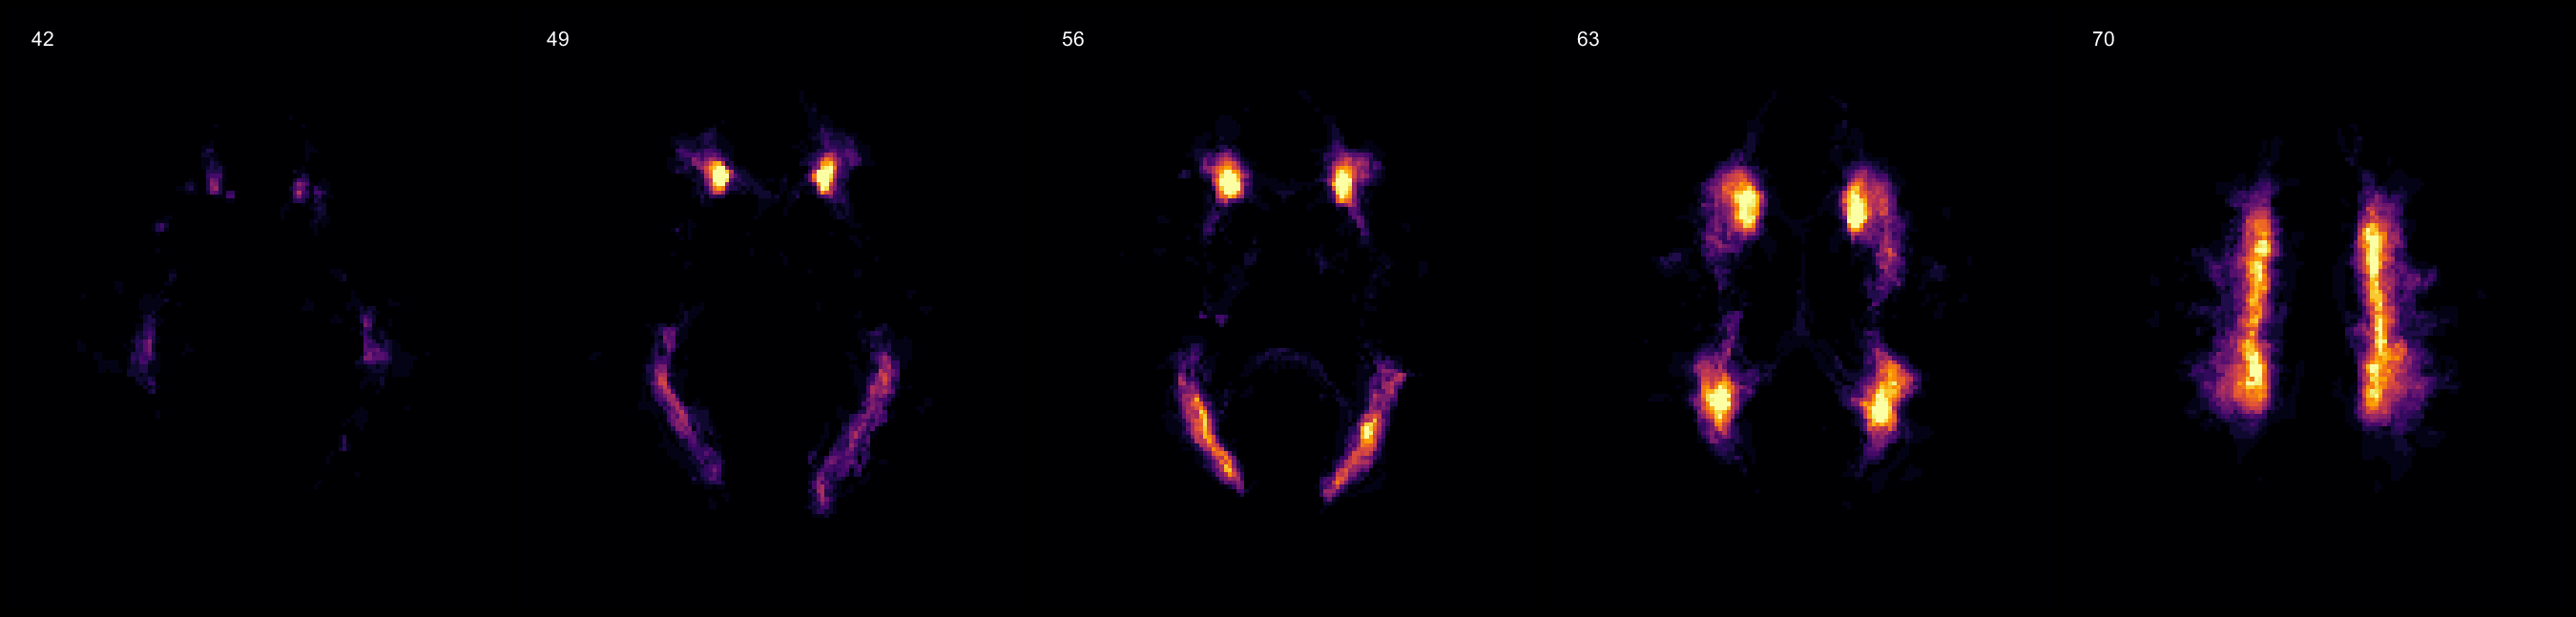
\includegraphics[height=\sliceheight]{rawthropt-tp.png} 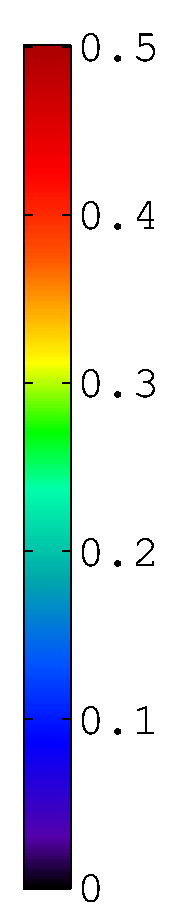
\includegraphics[height=\sliceheight]{cbar-NIH3-0-05}\end{subfigureside}\\[0.5em]
%    \begin{subfigureside}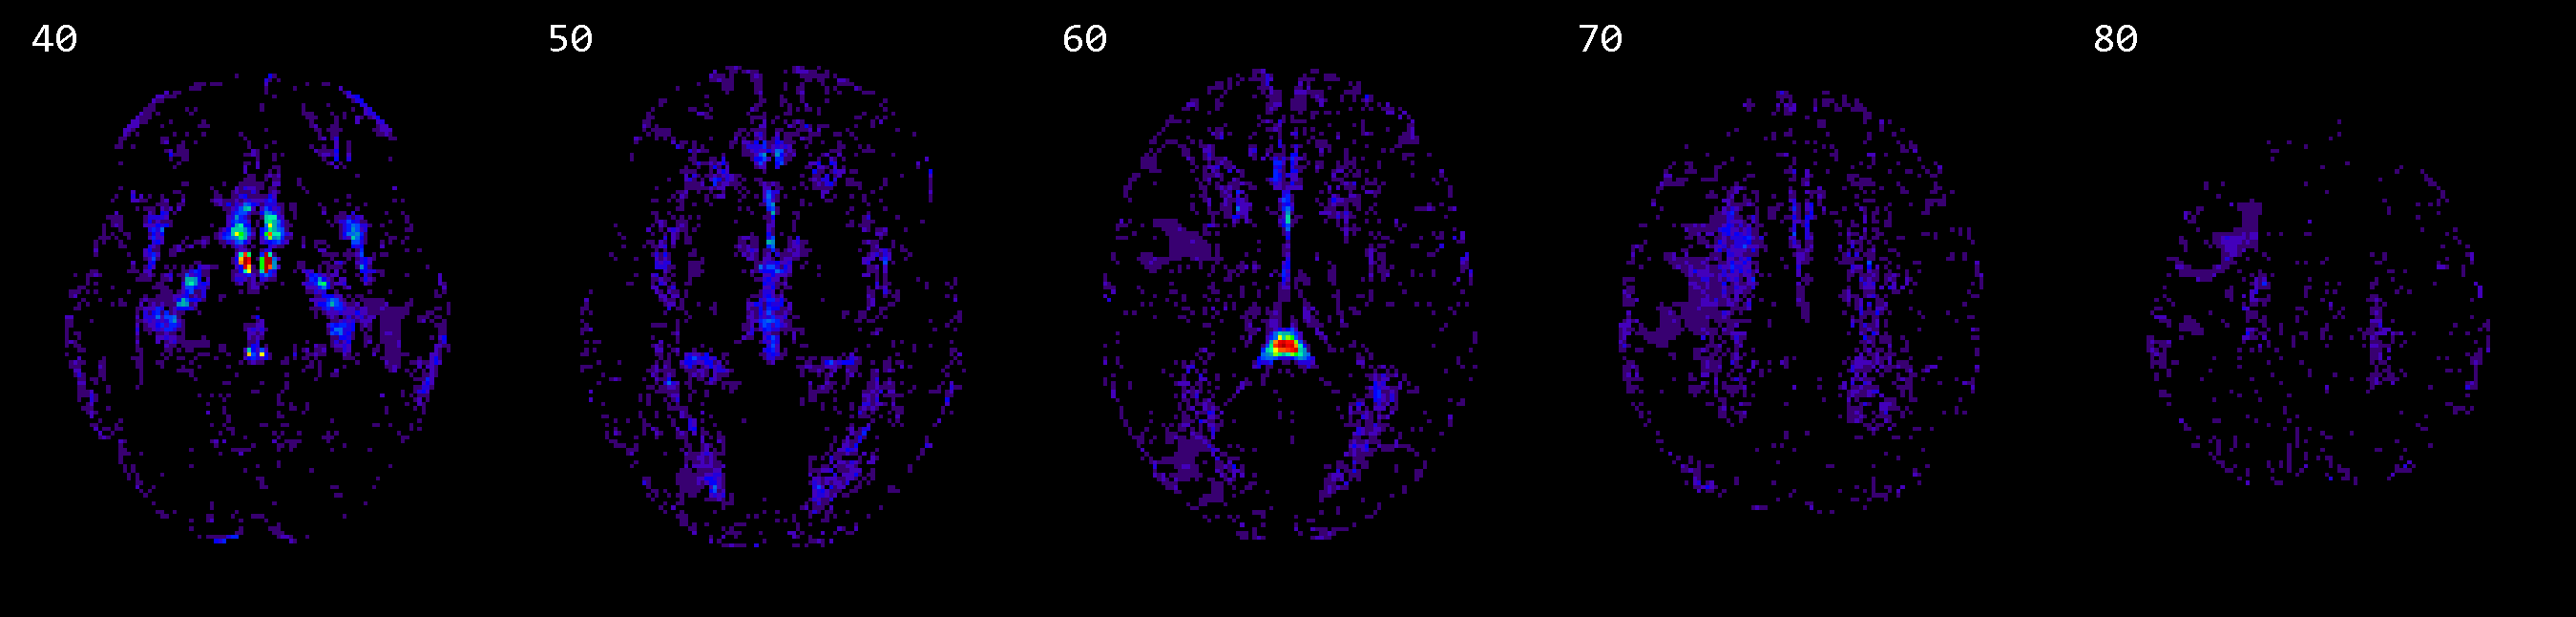
\includegraphics[height=\sliceheight]{rawthropt-fp.png} 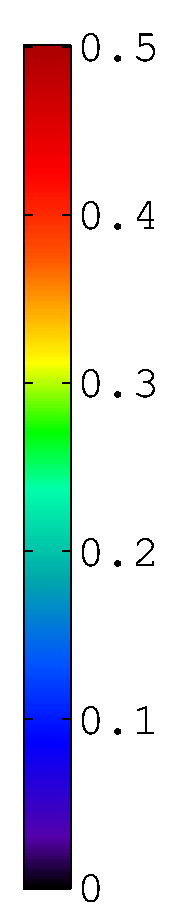
\includegraphics[height=\sliceheight]{cbar-NIH3-0-05}\end{subfigureside}\\[0.5em]
%    \begin{subfigureside}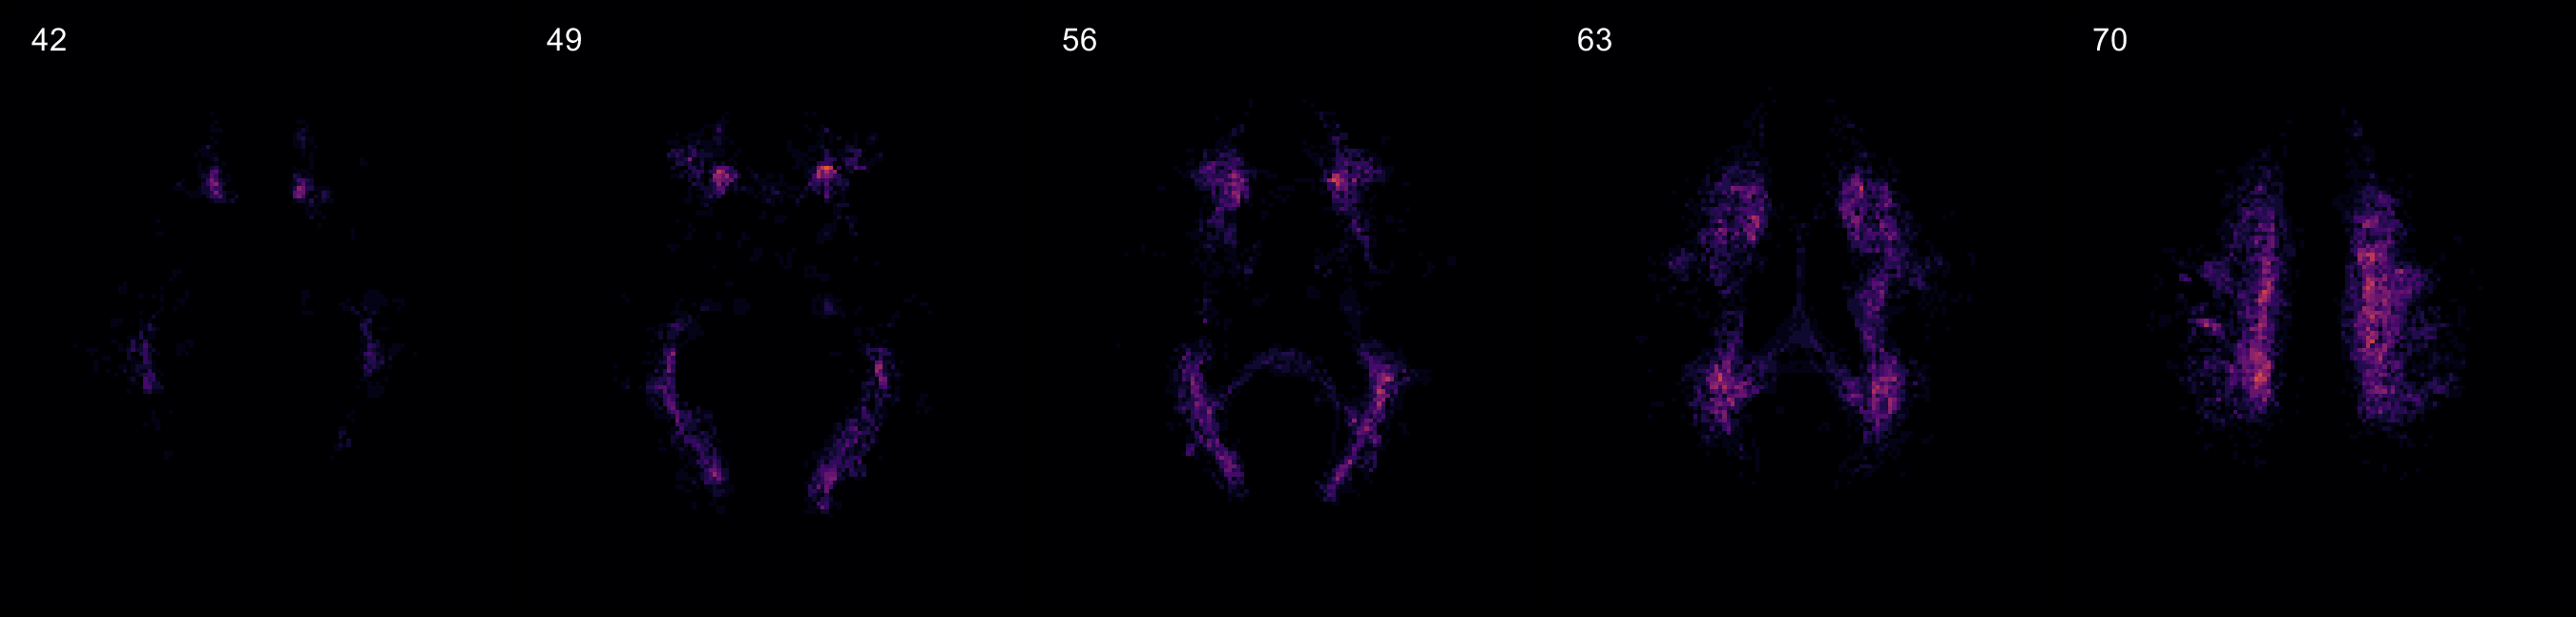
\includegraphics[height=\sliceheight]{rawthropt-fn.png} 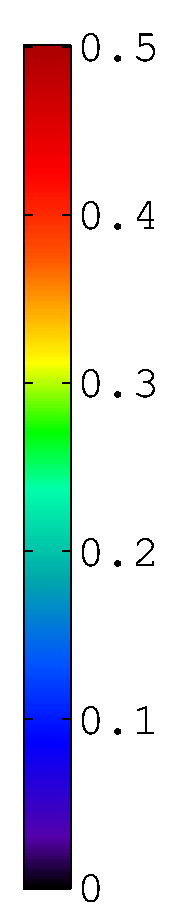
\includegraphics[height=\sliceheight]{cbar-NIH3-0-05}\end{subfigureside}\\[0.5em]
%    \caption{}
%  \end{figure}
% ---
%\begin{figure}\centering
%  \begin{minipage}{6cm}
%    \begin{subfigure}{\textwidth}
%      \centering\subcaption{Original}\label{fig:m08-rev-o}
%      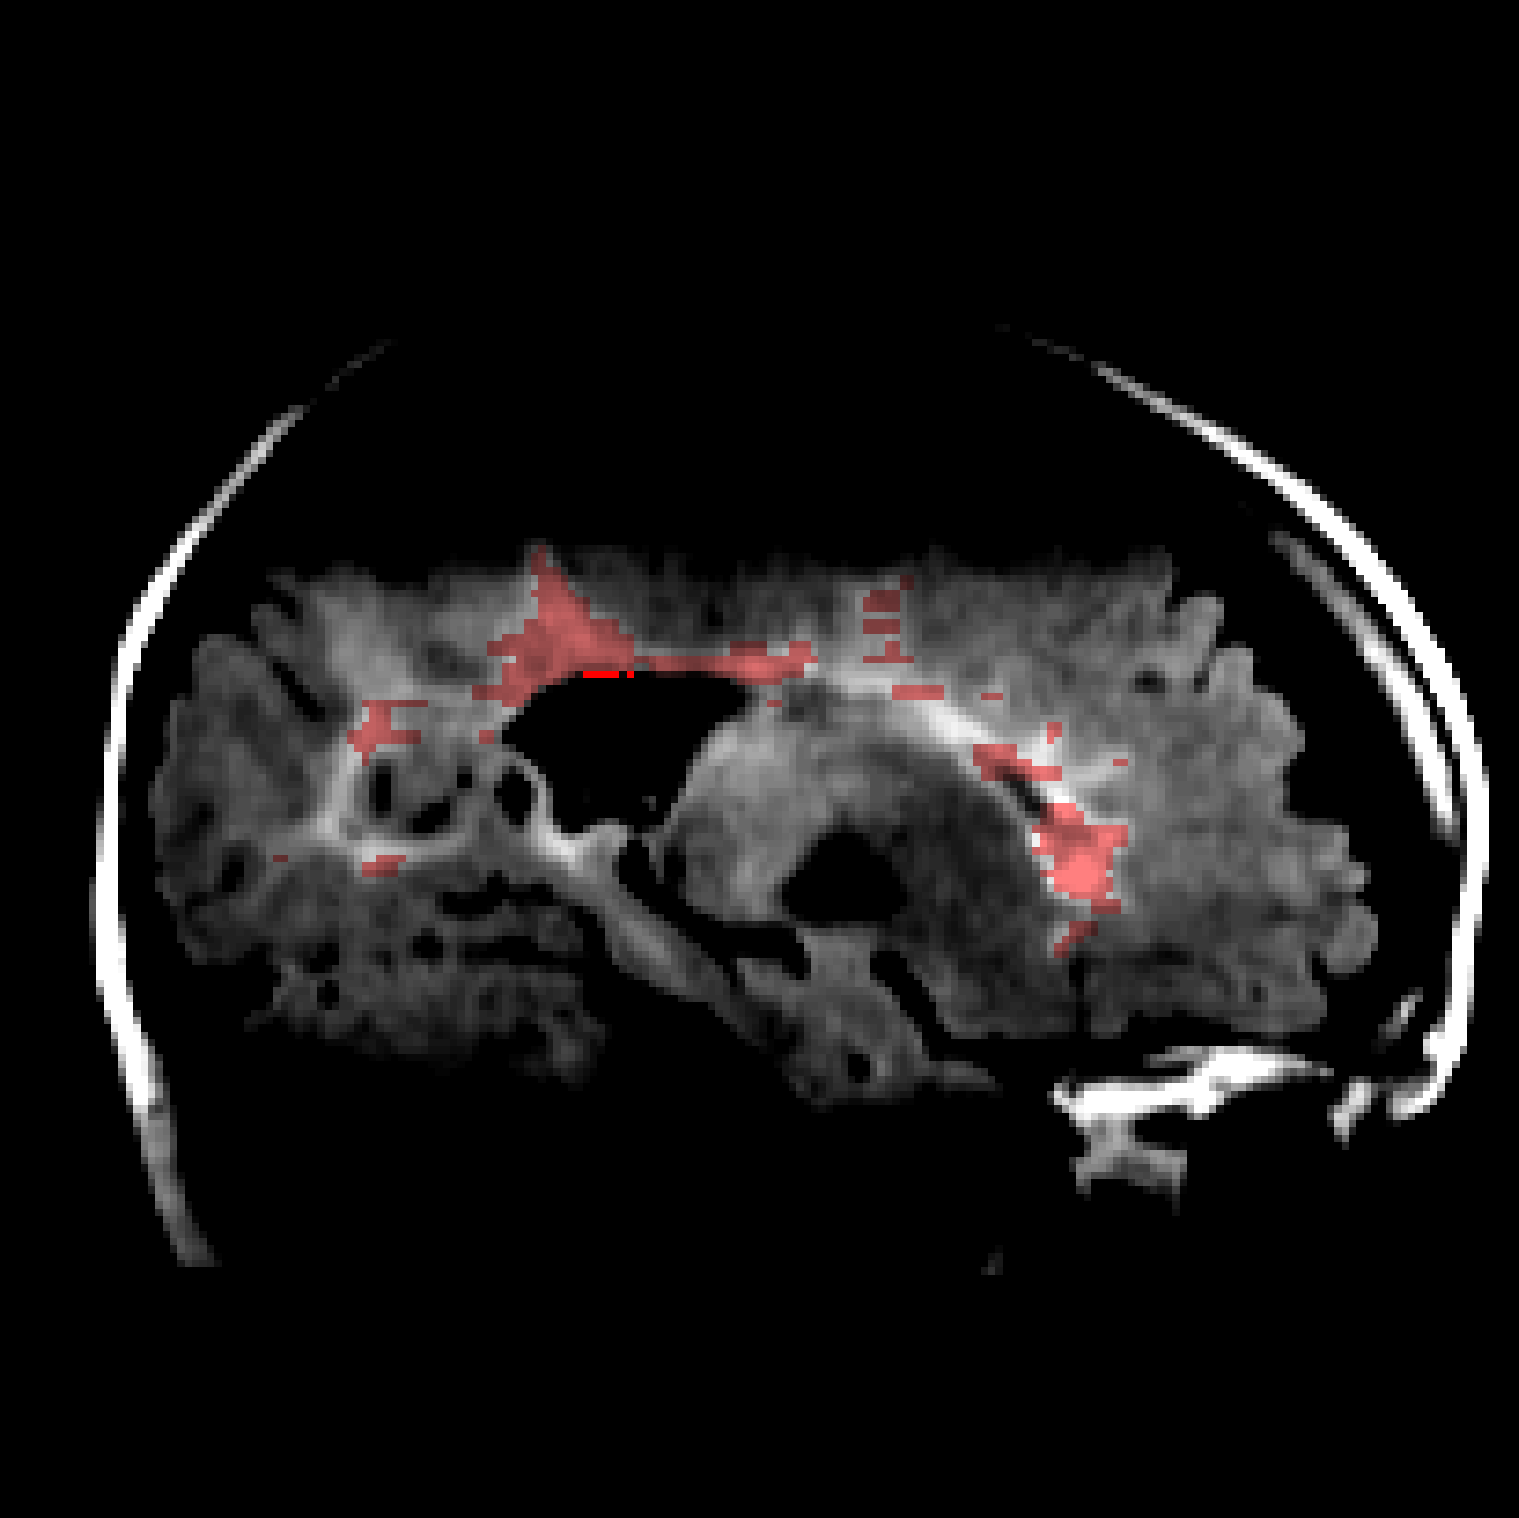
\includegraphics[height=6cm]{m08rev-01-d2-z146-o}\\[0.2em]
%      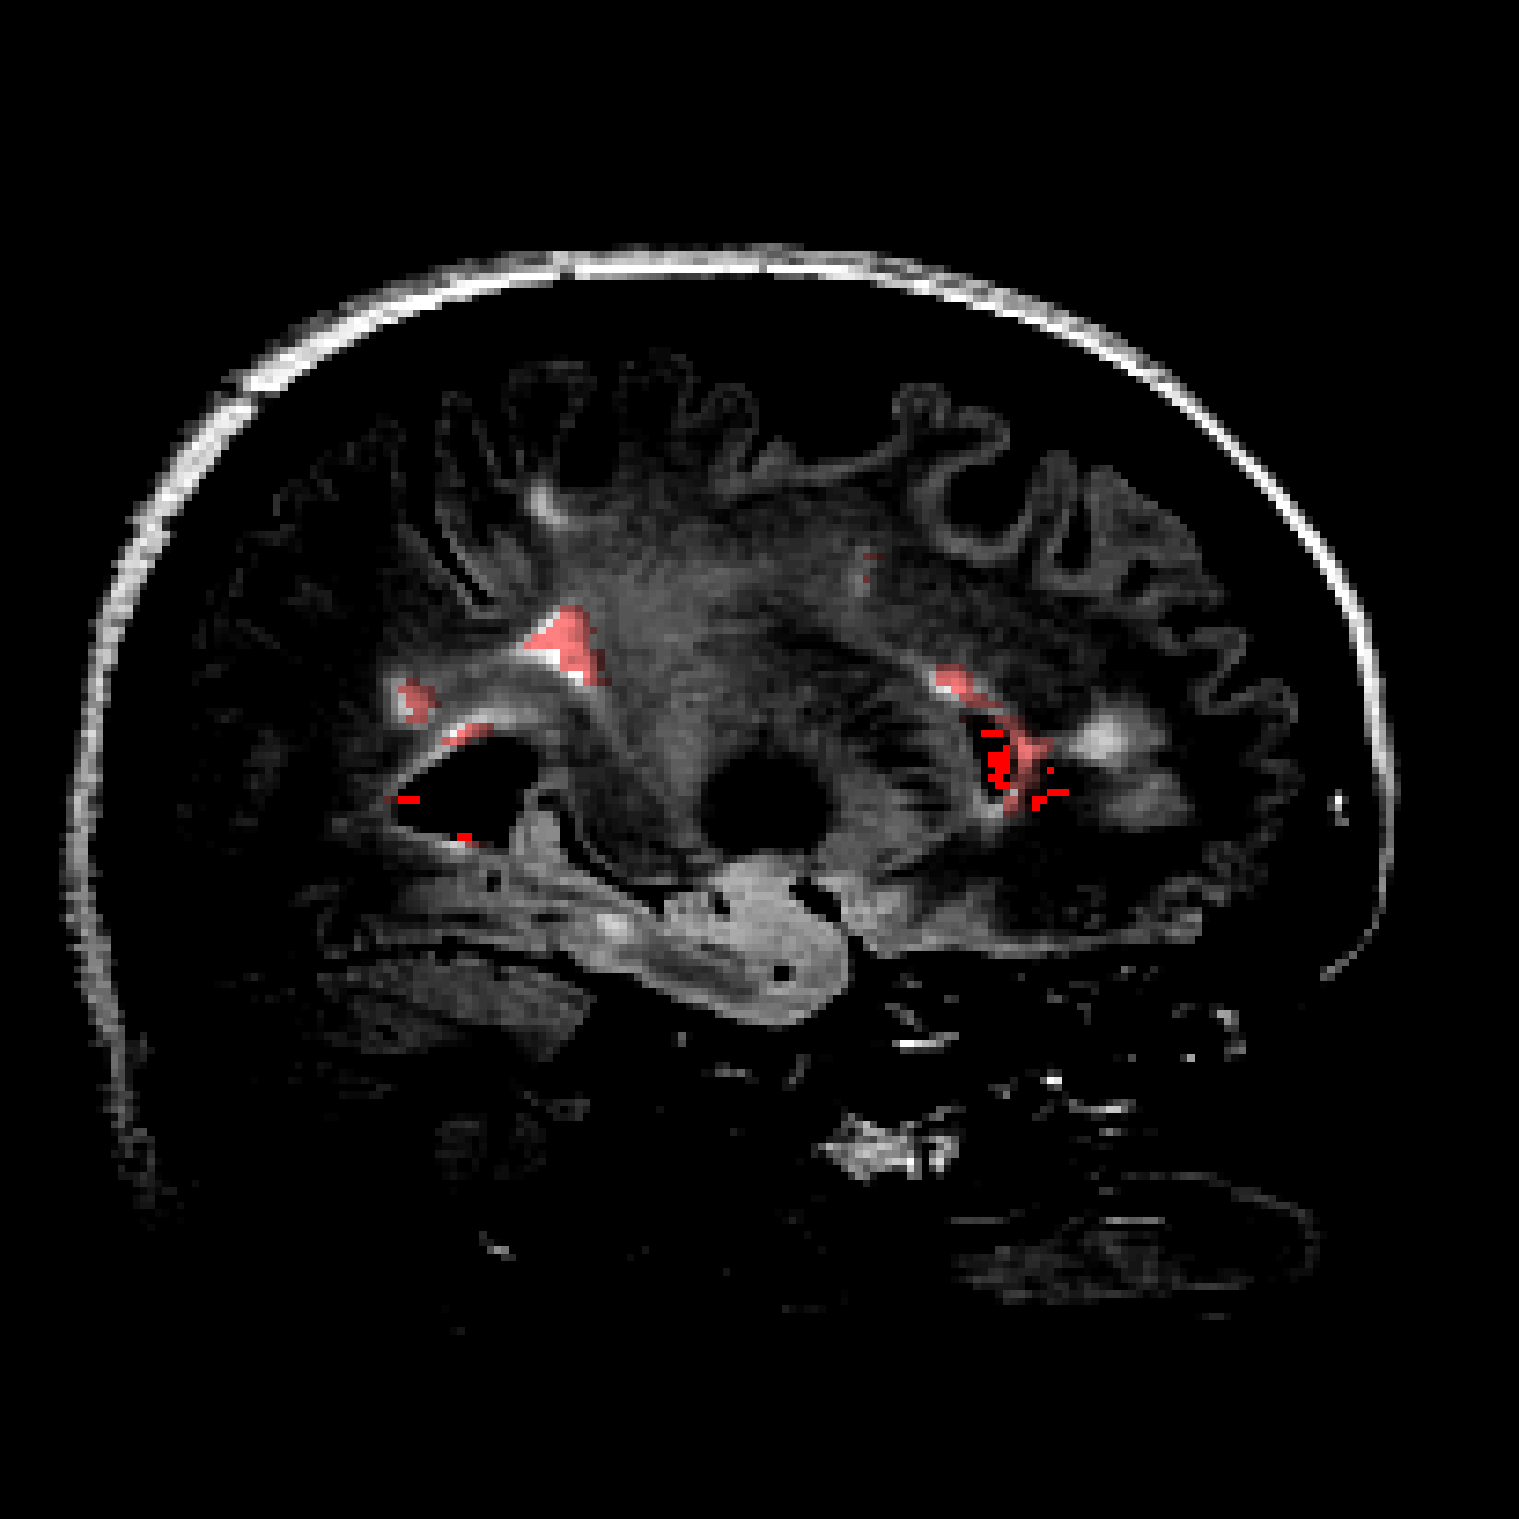
\includegraphics[height=6cm]{m08rev-05-d2-z107-o}\\[0.2em]
%      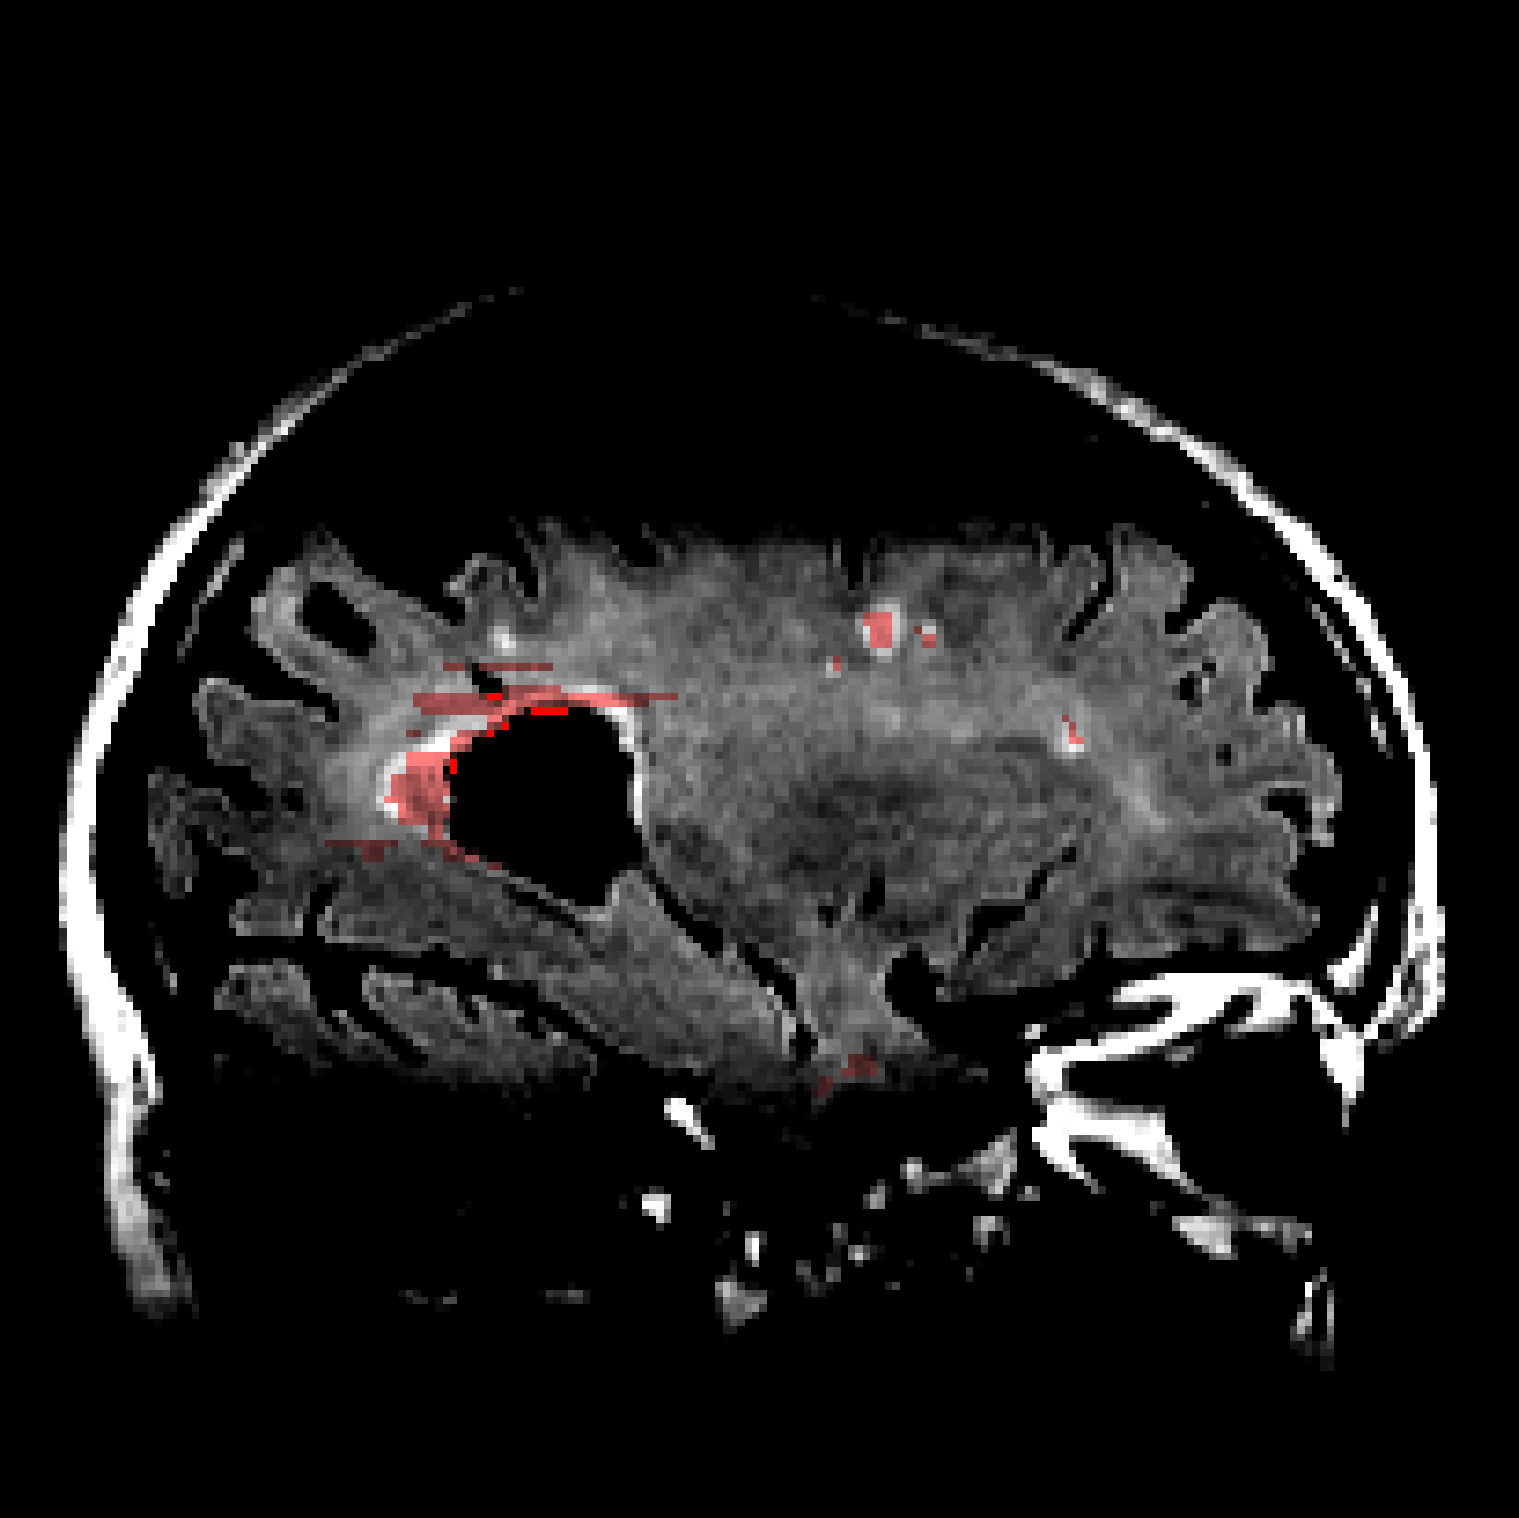
\includegraphics[height=6cm]{m08rev-06-d2-z101-o}
%    \end{subfigure}
%  \end{minipage}
%  \begin{minipage}{6cm}
%    \begin{subfigure}{\textwidth}
%      \centering\subcaption{Revision}\label{fig:m08-rev-r}
%      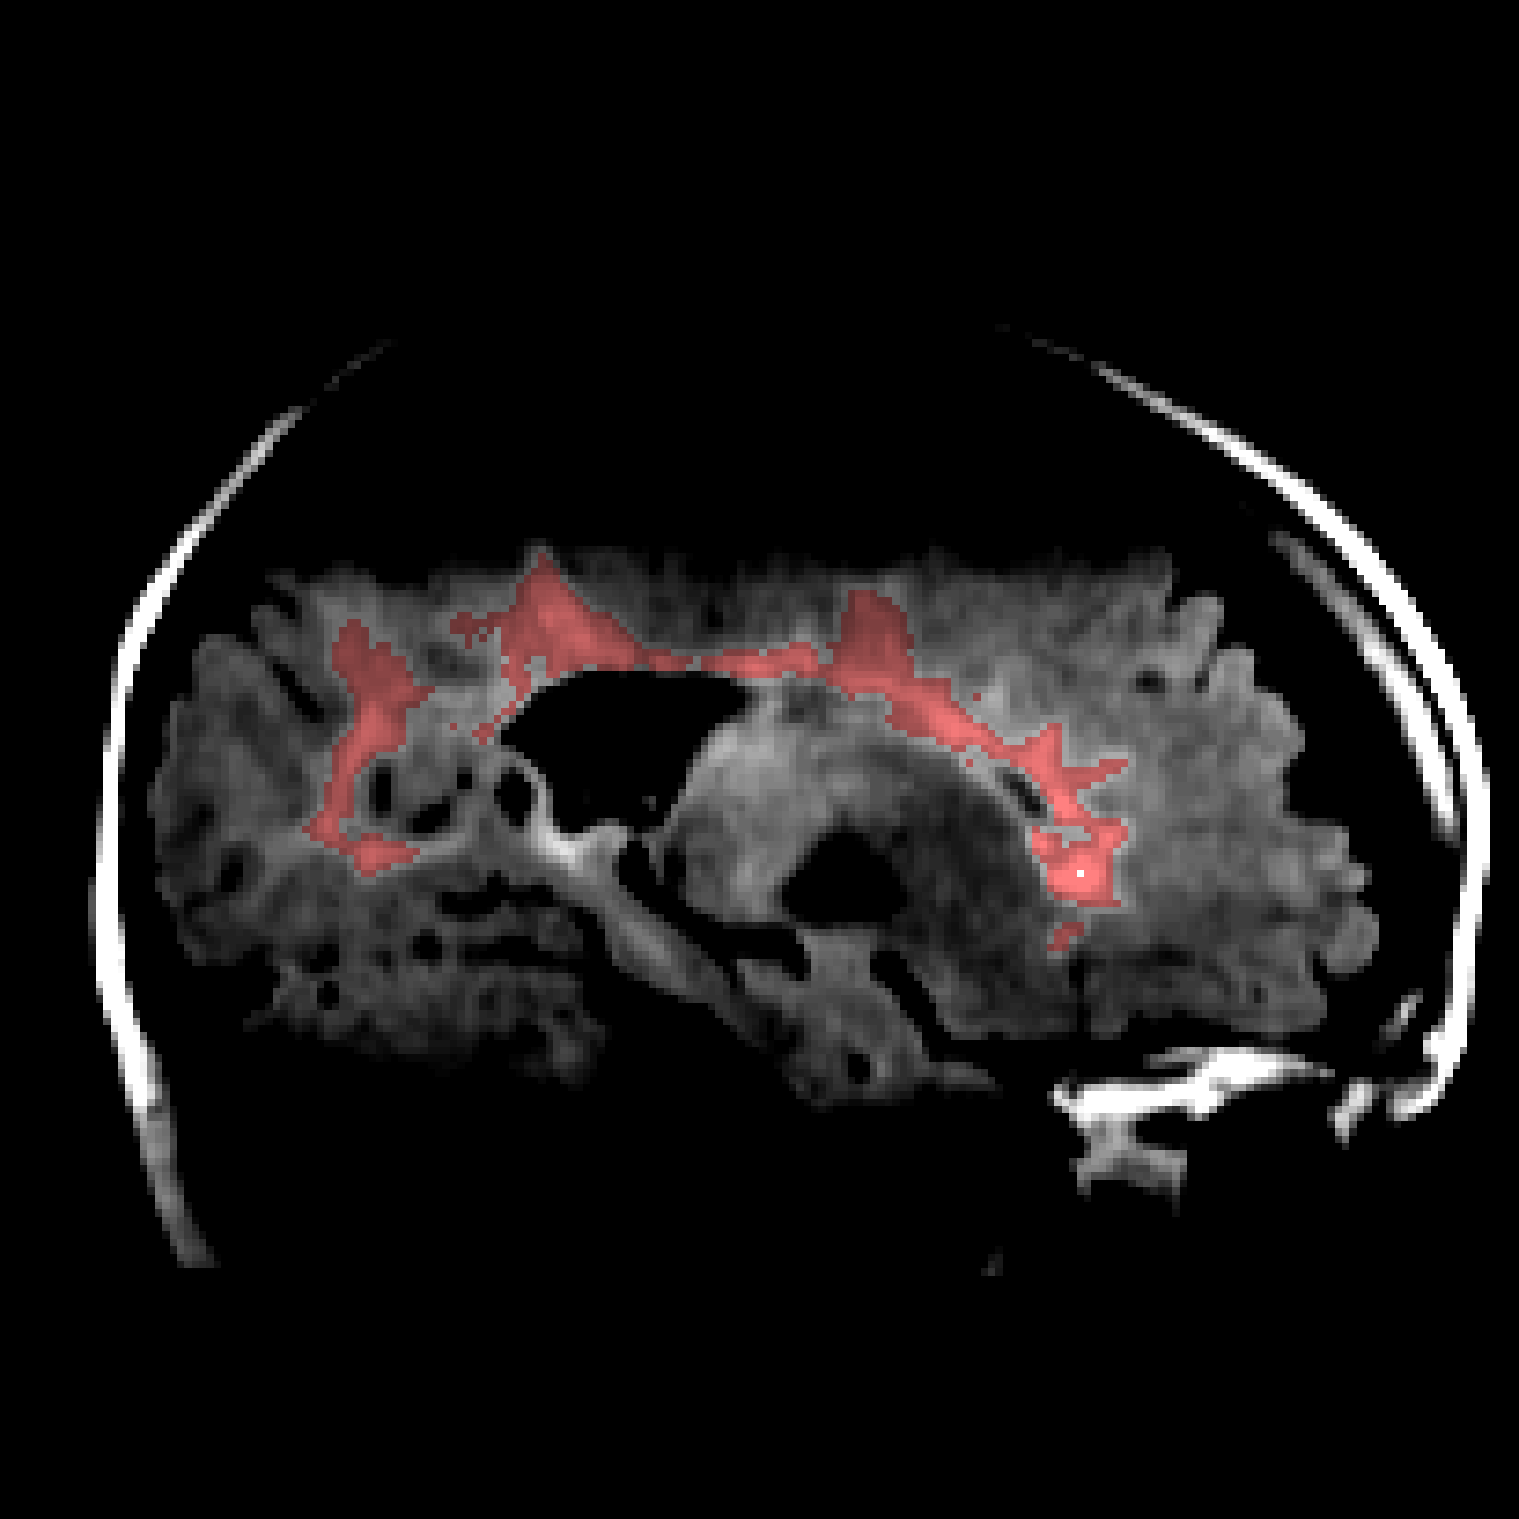
\includegraphics[height=6cm]{m08rev-01-d2-z146-r}\makebox[0pt][r]{\textcolor{white}{ CHB 01 }}\\[0.2em]
%      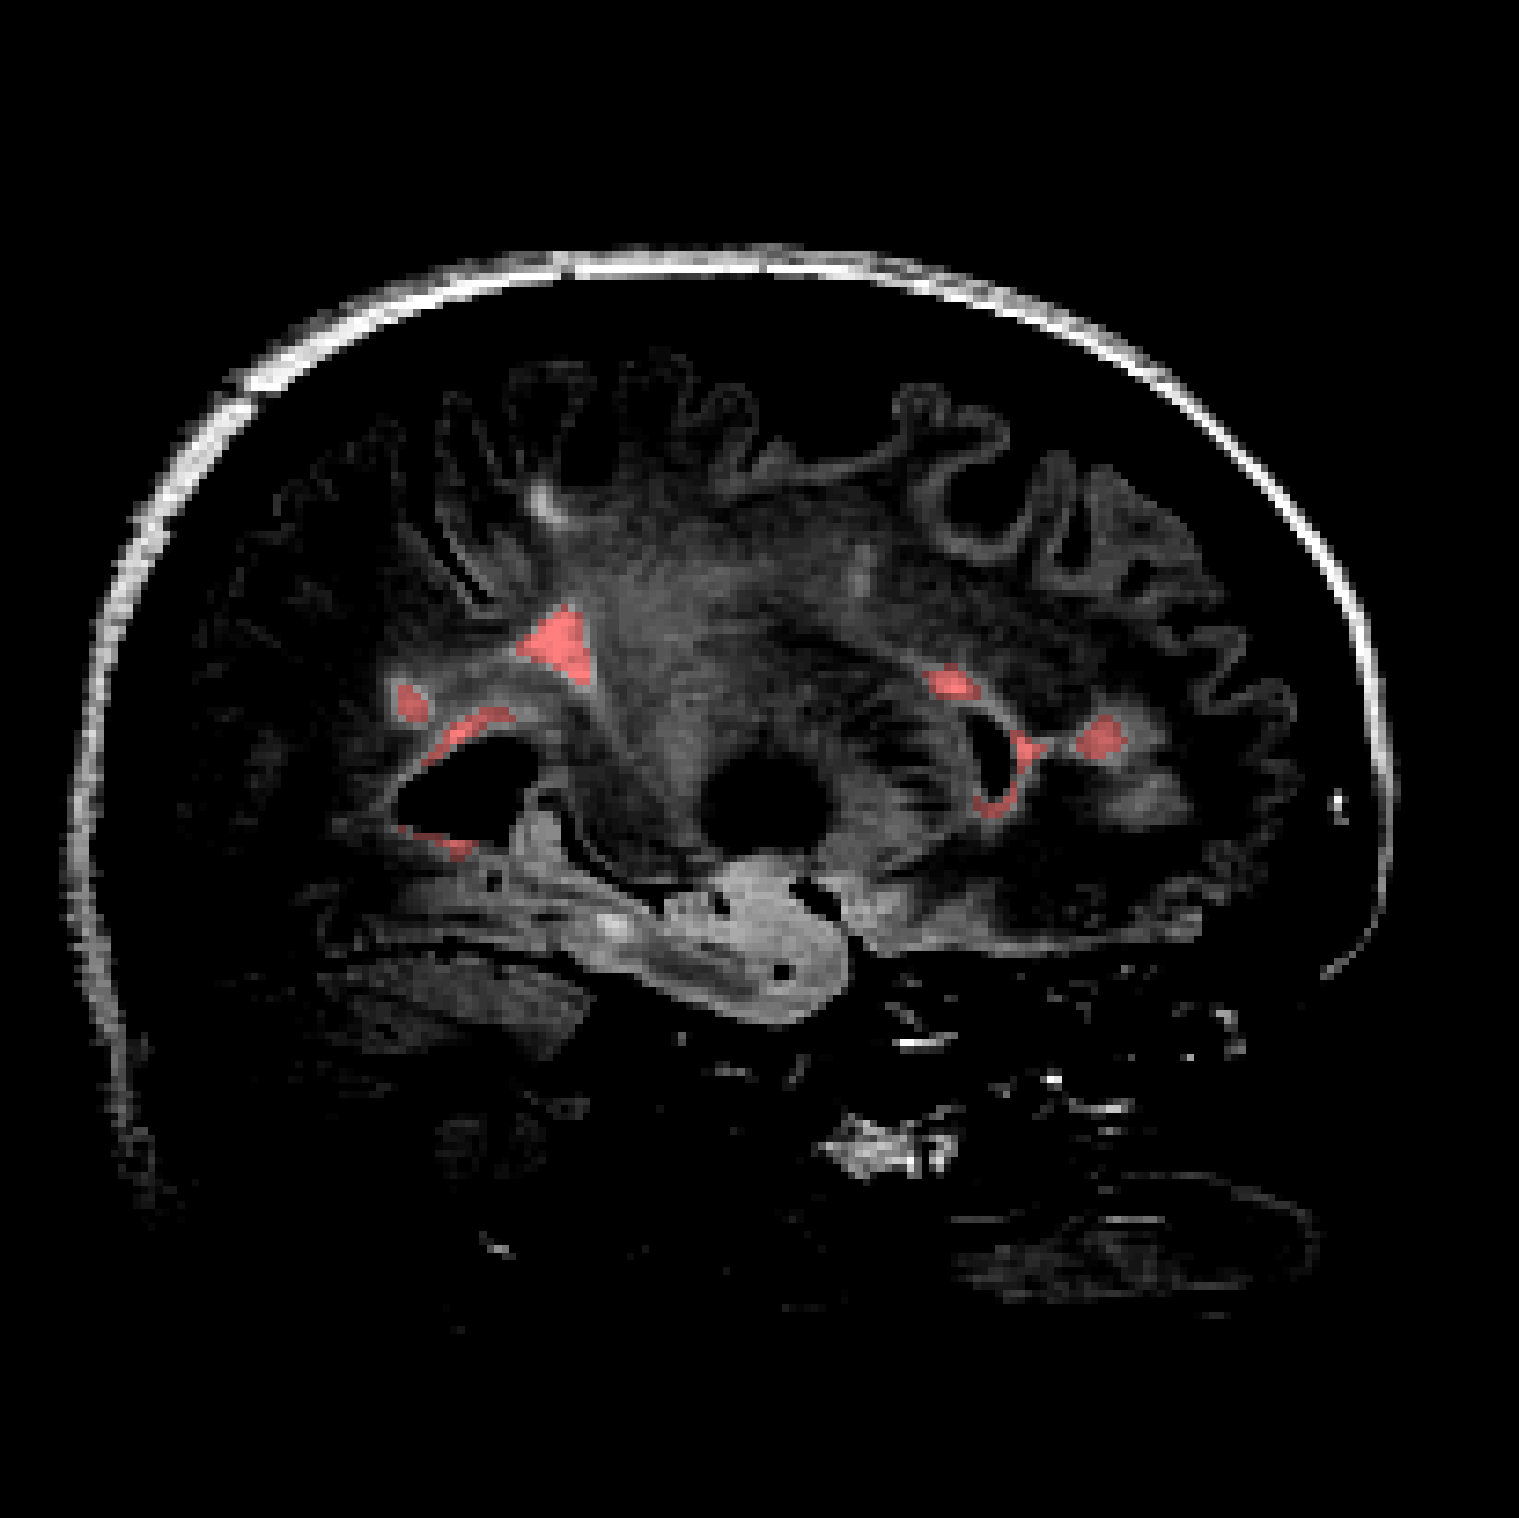
\includegraphics[height=6cm]{m08rev-05-d2-z107-r}\makebox[0pt][r]{\textcolor{white}{ CHB 05 }}\\[0.2em]
%      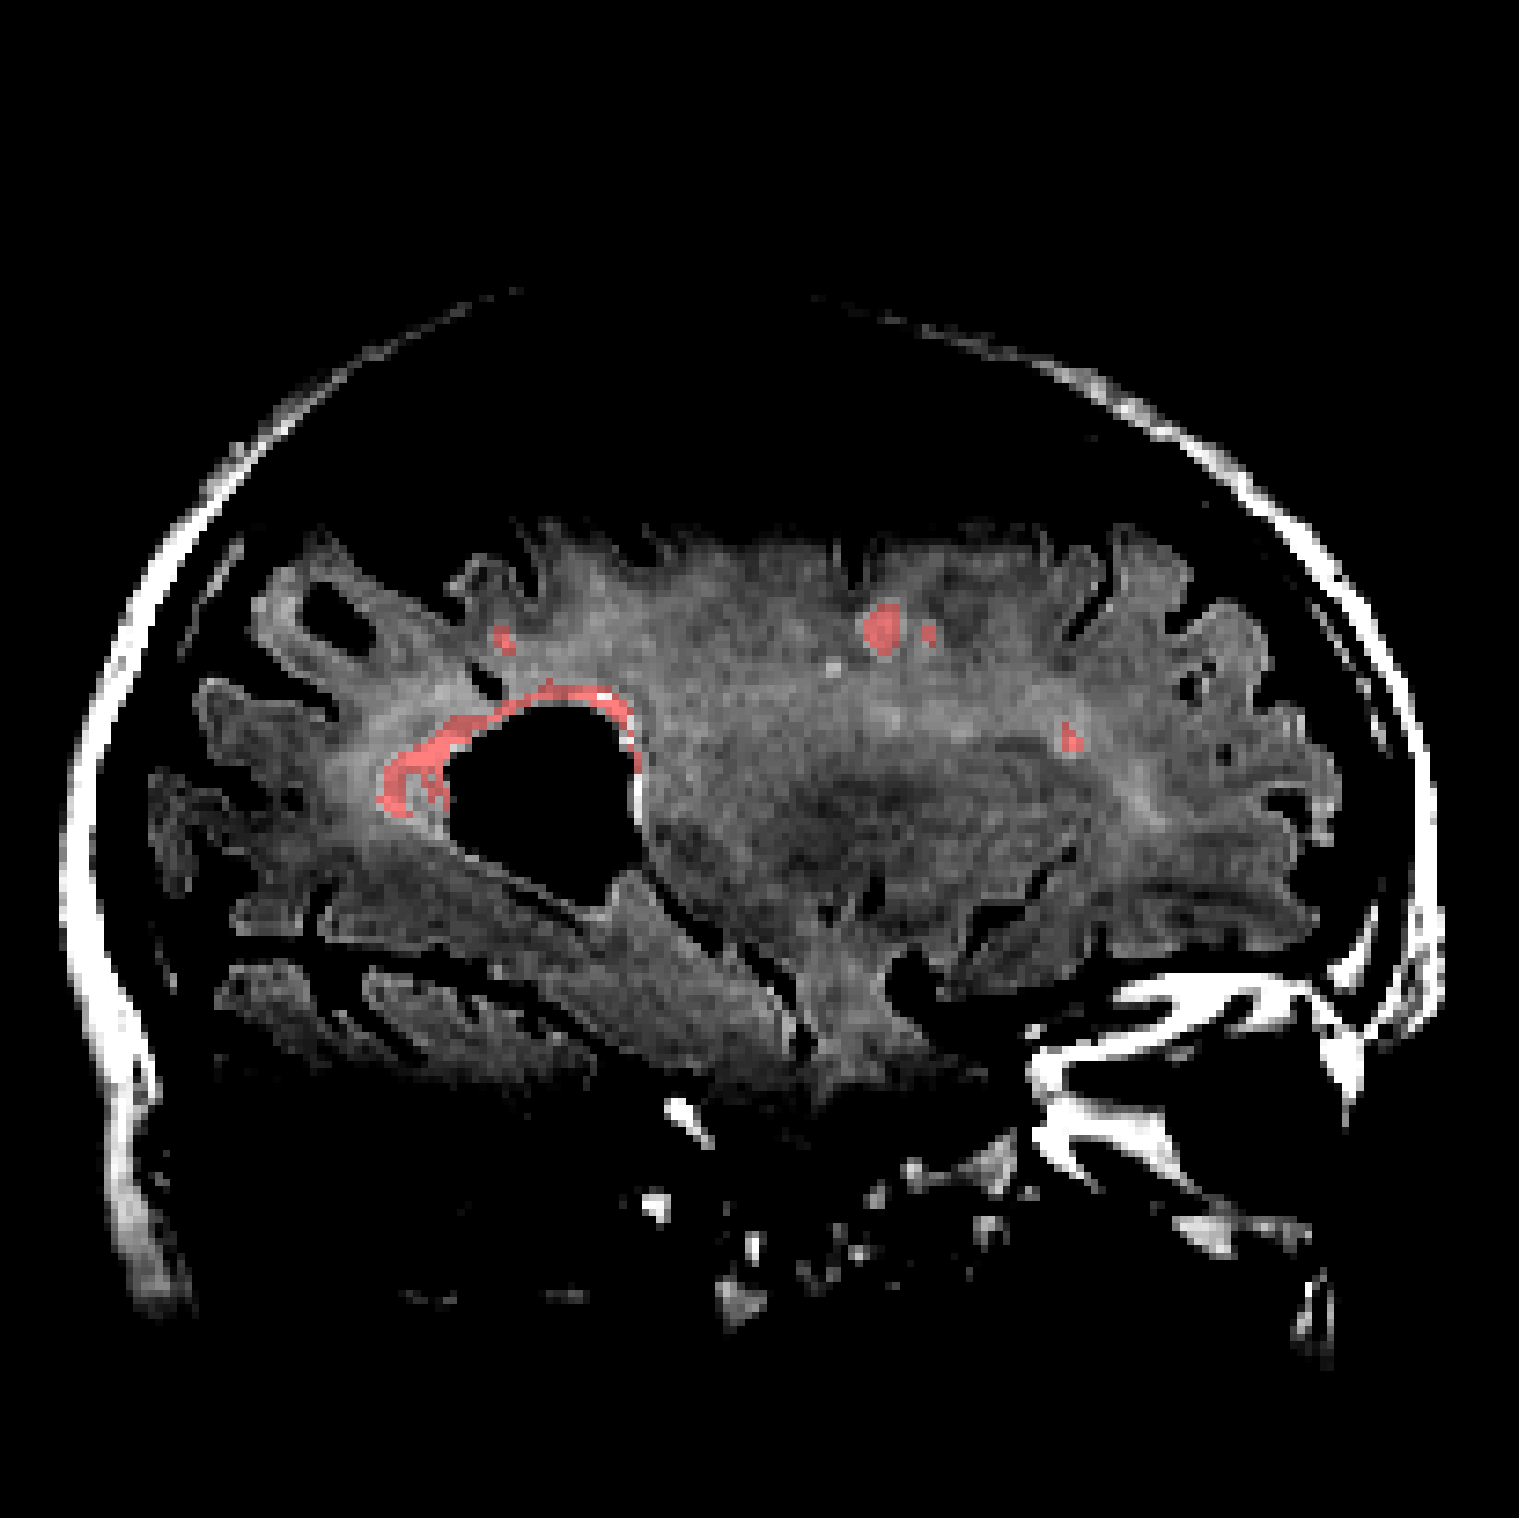
\includegraphics[height=6cm]{m08rev-06-d2-z101-r}\makebox[0pt][r]{\textcolor{white}{ CHB 06 }}
%    \end{subfigure}
%  \end{minipage}
%\end{figure}
% ---
%\begin{singlespace}
%\begin{table}[H]
%  \begin{tabular}{lll}
%  	\hline
%  	\multicolumn{3}{l}{Variables}                                                                       \\ \hline
%  	$y$                   & feature                                              & $\in\Re$             \\
%  	$\tilde{y}$           & standardized feature                                 & $\in\Re$             \\
%  	$c$                   & true class                                           & $\in\{0,1\}$         \\
%  	$\hat{c}$             & estimated class                                      & $\in[0,1]$           \\
%  	$\beta$               & logistic model feature weight                        & $\in\Re$             \\ \hline
%  	\multicolumn{3}{l}{Indexing -- e.g. arbitrary variable $a$}                                         \\ \hline
%  	$k$                   & feature index                                        & $\in \{1,\dots,K\}$  \\
%  	$n$                   & subject index                                        & $\in \{1,\dots,N\}$  \\
%  	$x$                   & spatial location                                     & $= [\xxx]$           \\
%  	$a_n^k(x)$            & $k$\ss{th} feature; $n$\ss{th} subject; location $x$ &                      \\ \hline
%  	\multicolumn{3}{l}{Images \& sets -- e.g. arbitrary variable $a$}                                   \\ \hline
%  	$a$                   & one voxel, one feature, one subject                  &                      \\
%  	$\bm{a}$              & one voxel, all features, one subject                 &                      \\
%  	$\mathrm{A}(x)$       & image in native space                                &                      \\
%  	$A(x)$                & image in standard space (MNI)                        &                      \\
%  	$\bm{A}(x)$           & image set: all features, one subject                 &                      \\
%  	$\mathcal{A}(x)$      & image set: one feature, all subjects                 &                      \\
%  	$\bm{\mathcal{A}}(x)$ & image superset: all features, all subjects           &                      \\ 
%    $\x{A}$               & full dataset: all features, subjects, voxels         &                      \\ \hline
%  \end{tabular}
%\end{table}
%\end{singlespace}
%\clearpage
%% __JK__ please forgive this strange notation for vectorization in x: \x{Y} -- any better ideas? I tried \vec{} but its confusing for the 3D matrices...
%First, the training data from all subjects -- features $\bm{\Y}(x)$, with $\Y^0=1$, and labels $\C(x)$ -- are sampled from nonzero locations in the MNI-space brain mask. These data are stored in two matrices $\x{Y}$ and $\x{C}$, with dimensions $[V,N,K+1]$ and $[V,N,1]$, respectively, where $V$ is the total number of nonzero voxels in the brain mask, $N$ is the number of subjects, and $K$ is the number of features. A similar matrix is constructed for the initial parameters $\bb^{(0)}(x)$, denoted $\x{B}^{(0)}$, with dimensions $[V,1,K+1]$. Let $\x{Y}_n^k$ denote the vector of data from all voxels for the $k$\ss{th} feature from the $n$\ss{th} subject, and so on for $\x{C}$ and $\x{B}$.
%\par
%In order to simplify subsequent gradient calculations, before the first iteration, the feature data are rectified according to the class labels, as in
%\begin{equation}
%\x{Y}_n^k =
%\begin{cases}
%+\x{Y}_n^k, & \x{C}_n \ge 0.5\\
%-\x{Y}_n^k, & \x{C}_n <  0.5\\
%\end{cases},\qquad\forall\et k \in \{1,\dots,K\}.
%\end{equation}
%Next, for a given iteration $t$, the following vectorized calculations yield the update matrix $\Delta\x{B}^{(t)}$. Regarding notation: 1) the iteration index ${}^{(t)}$ is omitted for clarity, 2) element-wise multiplication is denoted by $\circ$, and 3) the variable $K$ is now defined as $1$, since this is essential to the simplification.
%\begin{align}
%\x{S} &= \frac{1}{1+e^{\et\eta}},\qquad \eta = \x{B}^0 + \left(\x{B}^1\ep\x{Y}^1\right)\\
%\x{A} &= \x{S}\ep\left(1-\x{S}\right)\\
%\x{G} &= \nabla_{\x{B}}\L - \lambda\x{B} \nonumber \\
%      &= \left[\begin{array}{c}
%           \x{G}^1 \\ \x{G}^2
%         \end{array}\right] \nonumber \\
%      &= \left[\begin{array}{c}
%           \sum_{n=1}^{N}\left( \x{Y}_n^1\circ\x{S} \right) \\
%           \sum_{n=1}^{N}\left( \x{Y}_n^2\circ\x{S} \right)
%         \end{array}\right] - \lambda\left[\begin{array}{c} \x{B}^1 \\ \x{B}^2\end{array}\right]\\
%\x{H} &= \nabla_{\x{B}}^2\L -\lambda\x{I} \nonumber \\
%      &= \left[\begin{array}{cc}
%           \x{H}^{1,1} & \x{H}^{1,2} \\ \x{H}^{2,1} & \x{H}^{2,2}
%         \end{array}\right] \nonumber \\
%      &= \left[\begin{array}{cc}
%           \sum_{n=1}^{N}\left( \x{A}\circ\x{Y}_n^1\circ\x{Y}_n^1 \right) & 
%           \sum_{n=1}^{N}\left( \x{A}\circ\x{Y}_n^2\circ\x{Y}_n^1 \right) \\
%           \sum_{n=1}^{N}\left( \x{A}\circ\x{Y}_n^1\circ\x{Y}_n^2 \right) & 
%           \sum_{n=1}^{N}\left( \x{A}\circ\x{Y}_n^2\circ\x{Y}_n^2 \right)
%         \end{array}\right] - \lambda\left[\begin{array}{cc} 1 & \\ & 1\end{array}\right]\\
%\det{\x{H}} &= \left(\x{H}^{1,1}\circ\x{H}^{2,2}\right) - \left(\x{H}^{1,2}\circ\x{H}^{2,1}\right) \\
%\Delta\x{B} &= -\x{H}^{-1}\x{G} \nonumber \\
%      &= \dfrac{1}{\det{\x{H}}} \left[\begin{array}{cc}
%           \left(\x{H}^{2,2}\circ\x{G}^{1} - \x{H}^{2,1}\circ\x{G}^{2} \right) & 
%           \left(\x{H}^{1,2}\circ\x{G}^{2} - \x{H}^{1,1}\circ\x{G}^{1} \right)
%         \end{array}\right]^{T}
%\end{align}
% ---
%\begin{figure}
%  \centering
%%  \begin{subfigureside}[4cm]{Original}
%%    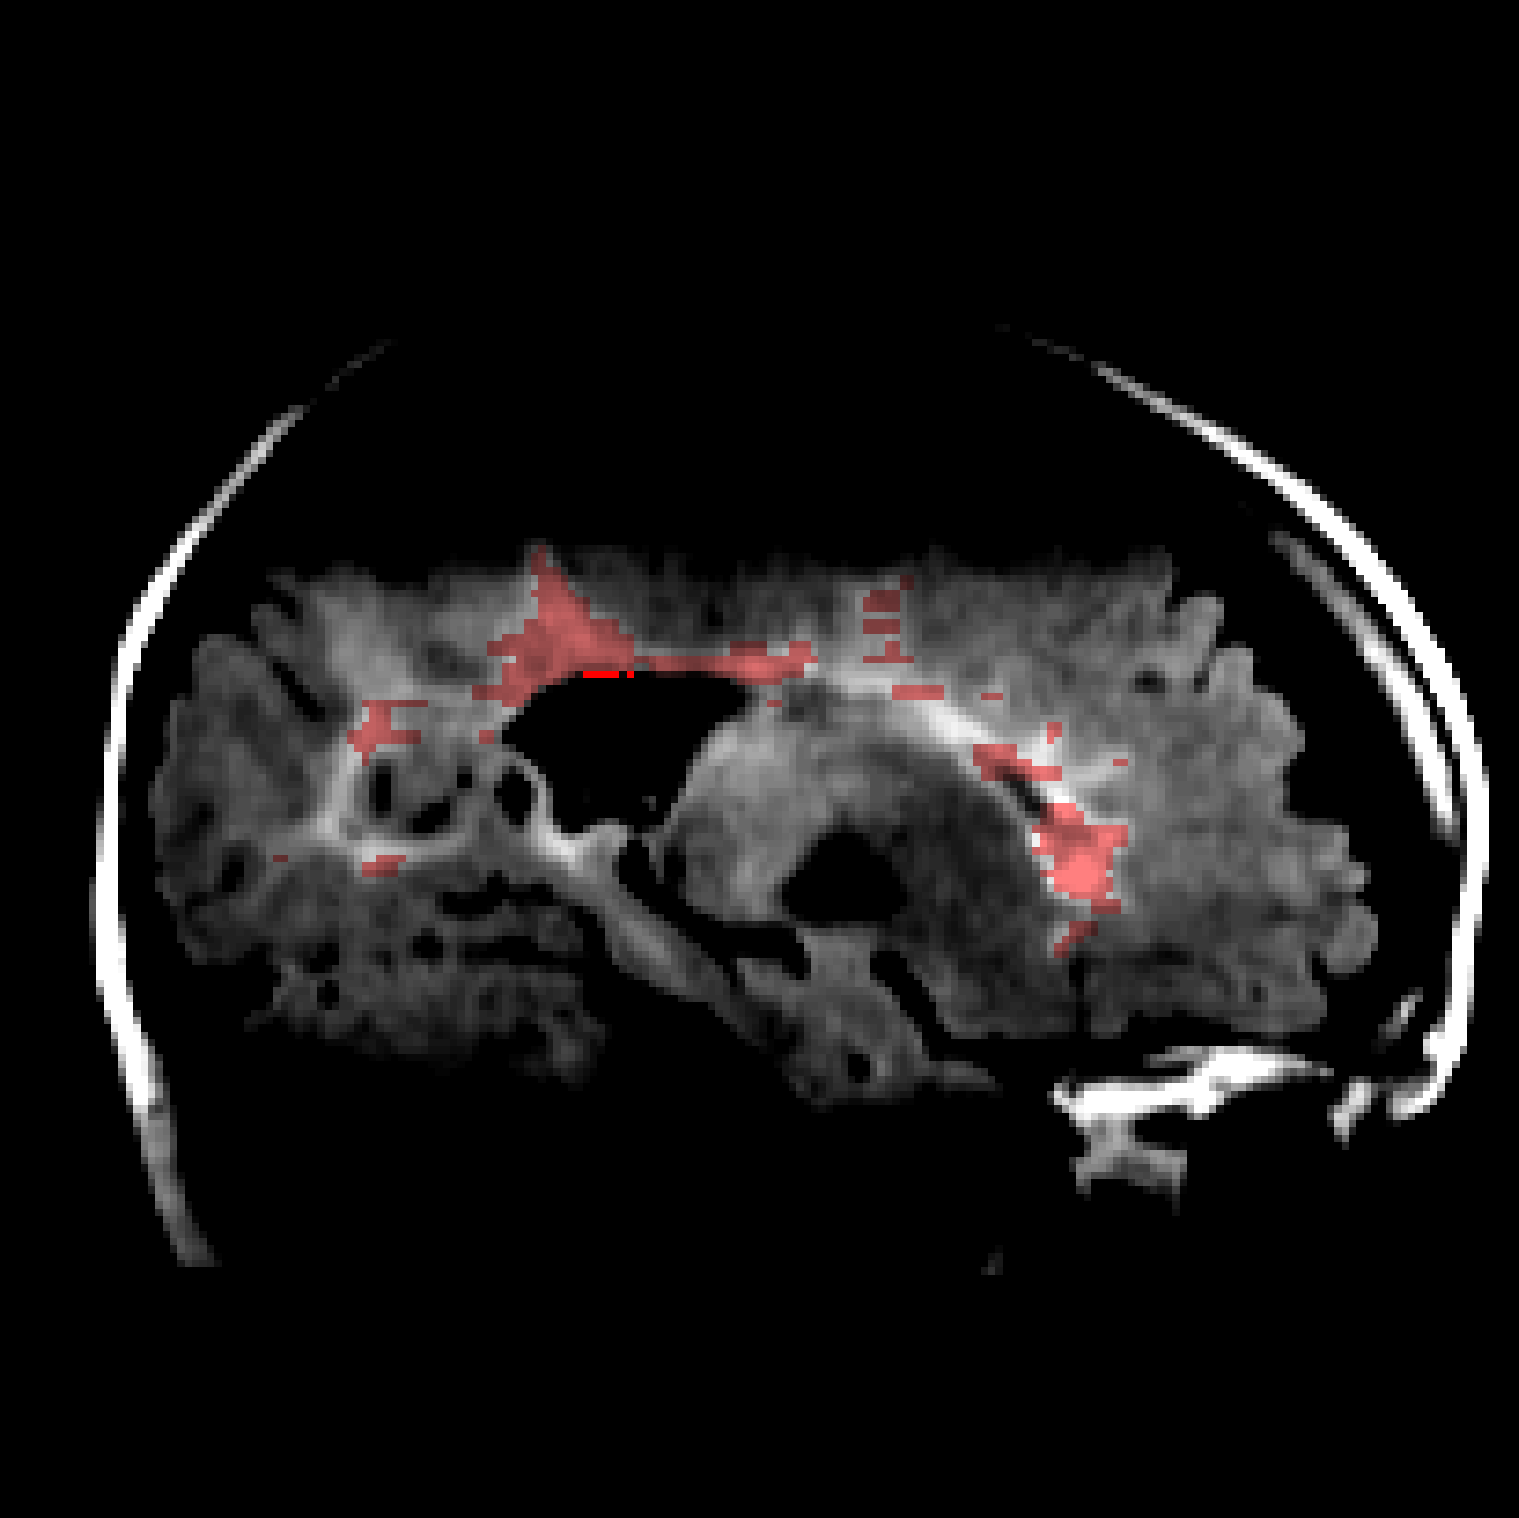
\includegraphics[height=4cm]{m08rev-01-d2-z146-o}
%%    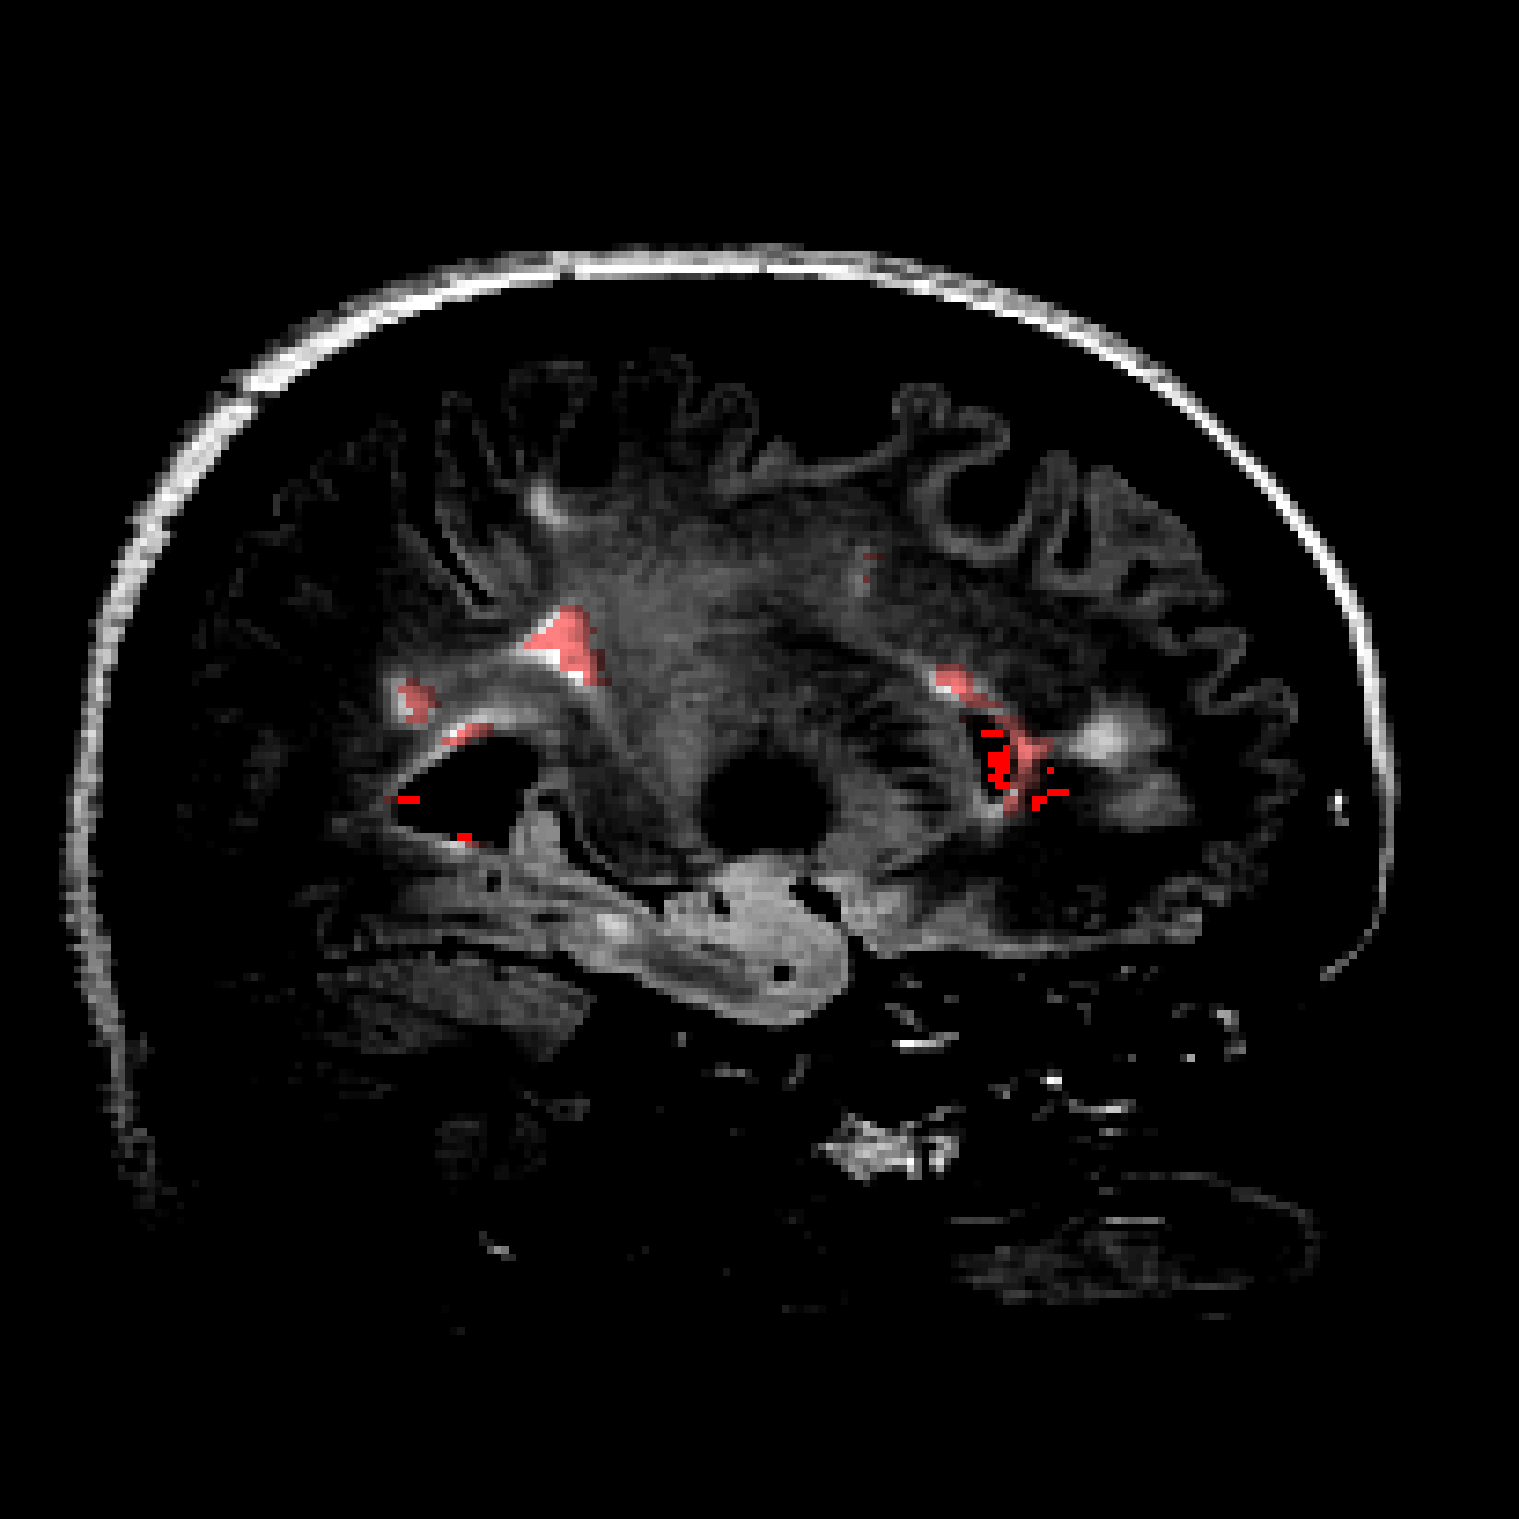
\includegraphics[height=4cm]{m08rev-05-d2-z107-o}
%%    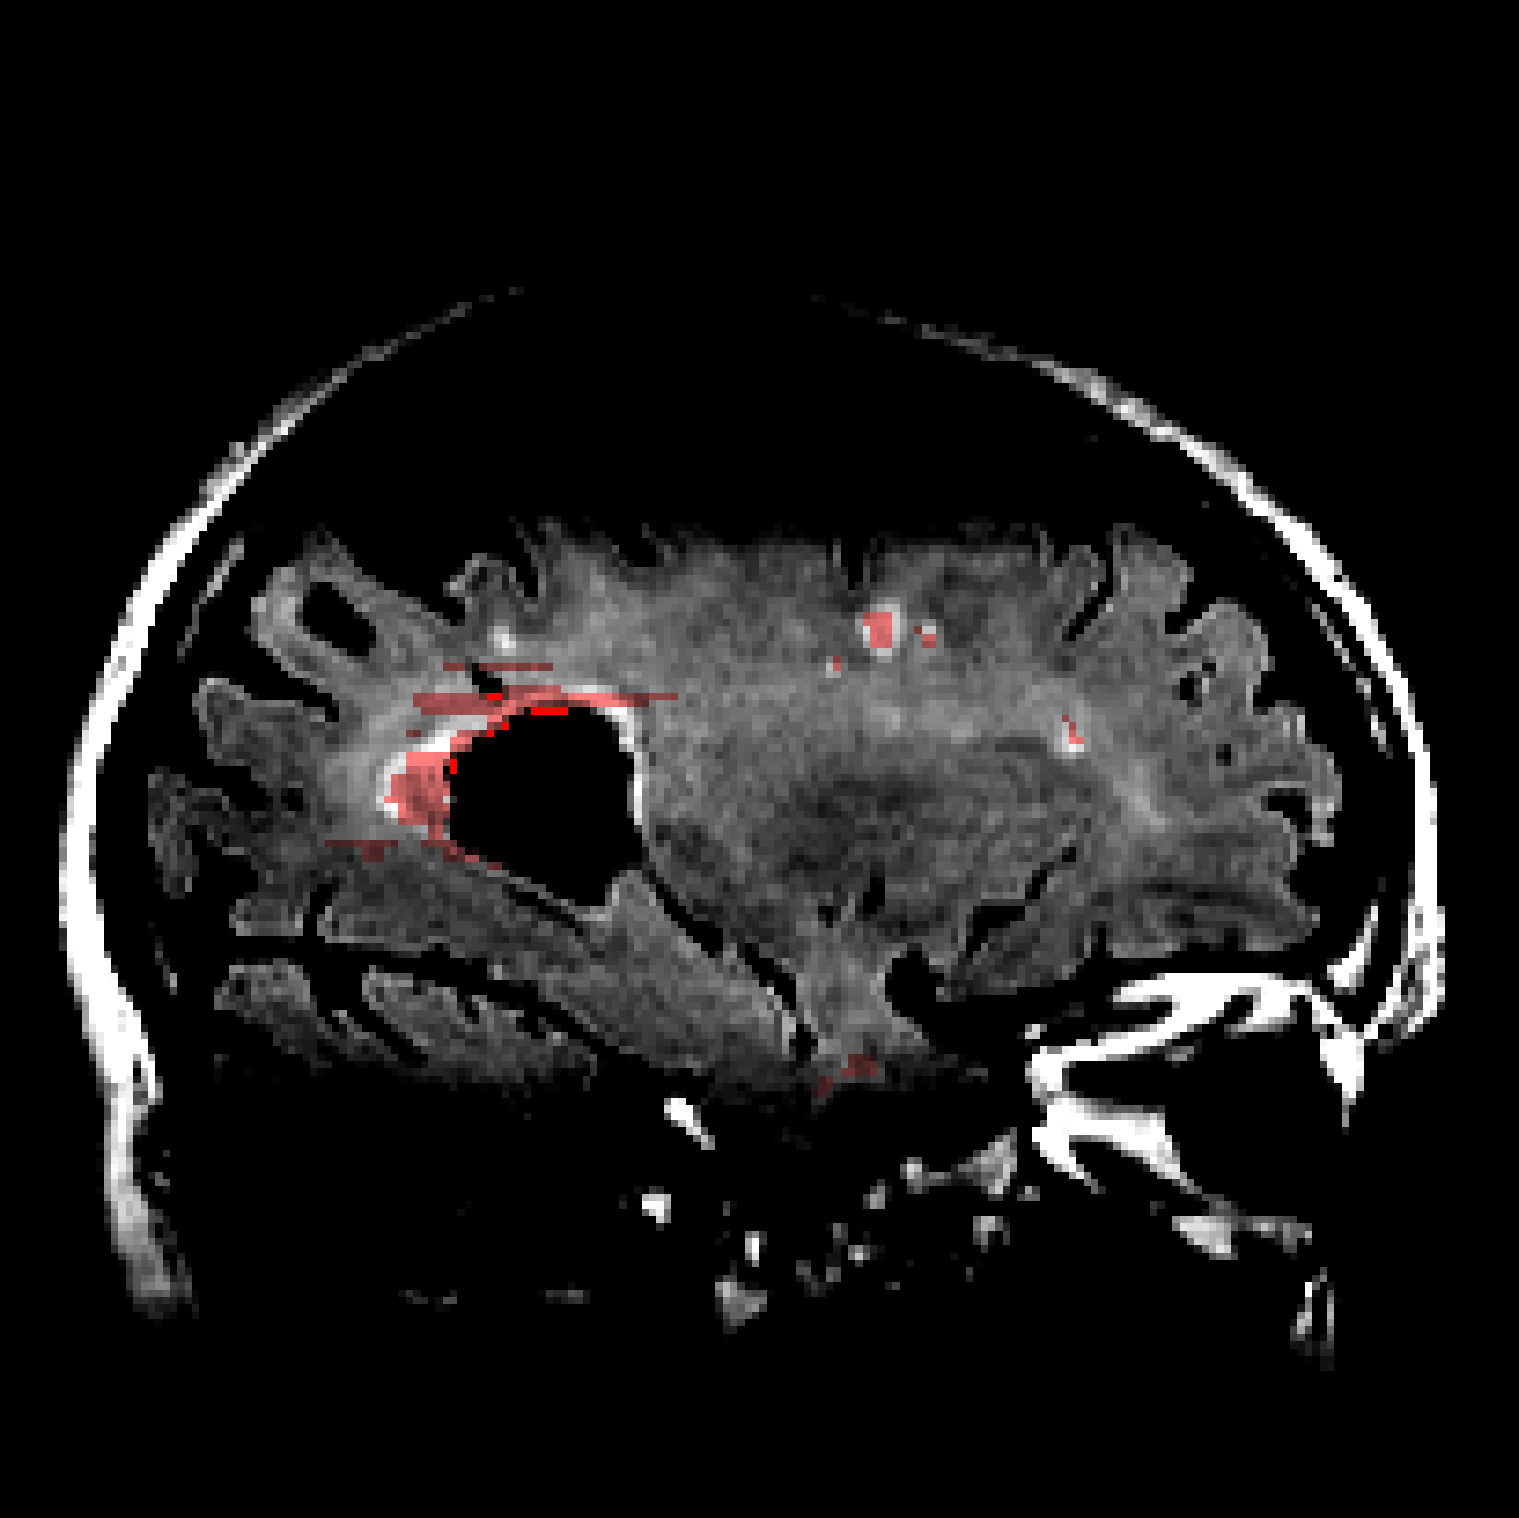
\includegraphics[height=4cm]{m08rev-06-d2-z101-o}
%%  \end{subfigureside}\\[0.25em]
%%  \begin{subfigureside}[4cm]{Revision}
%%    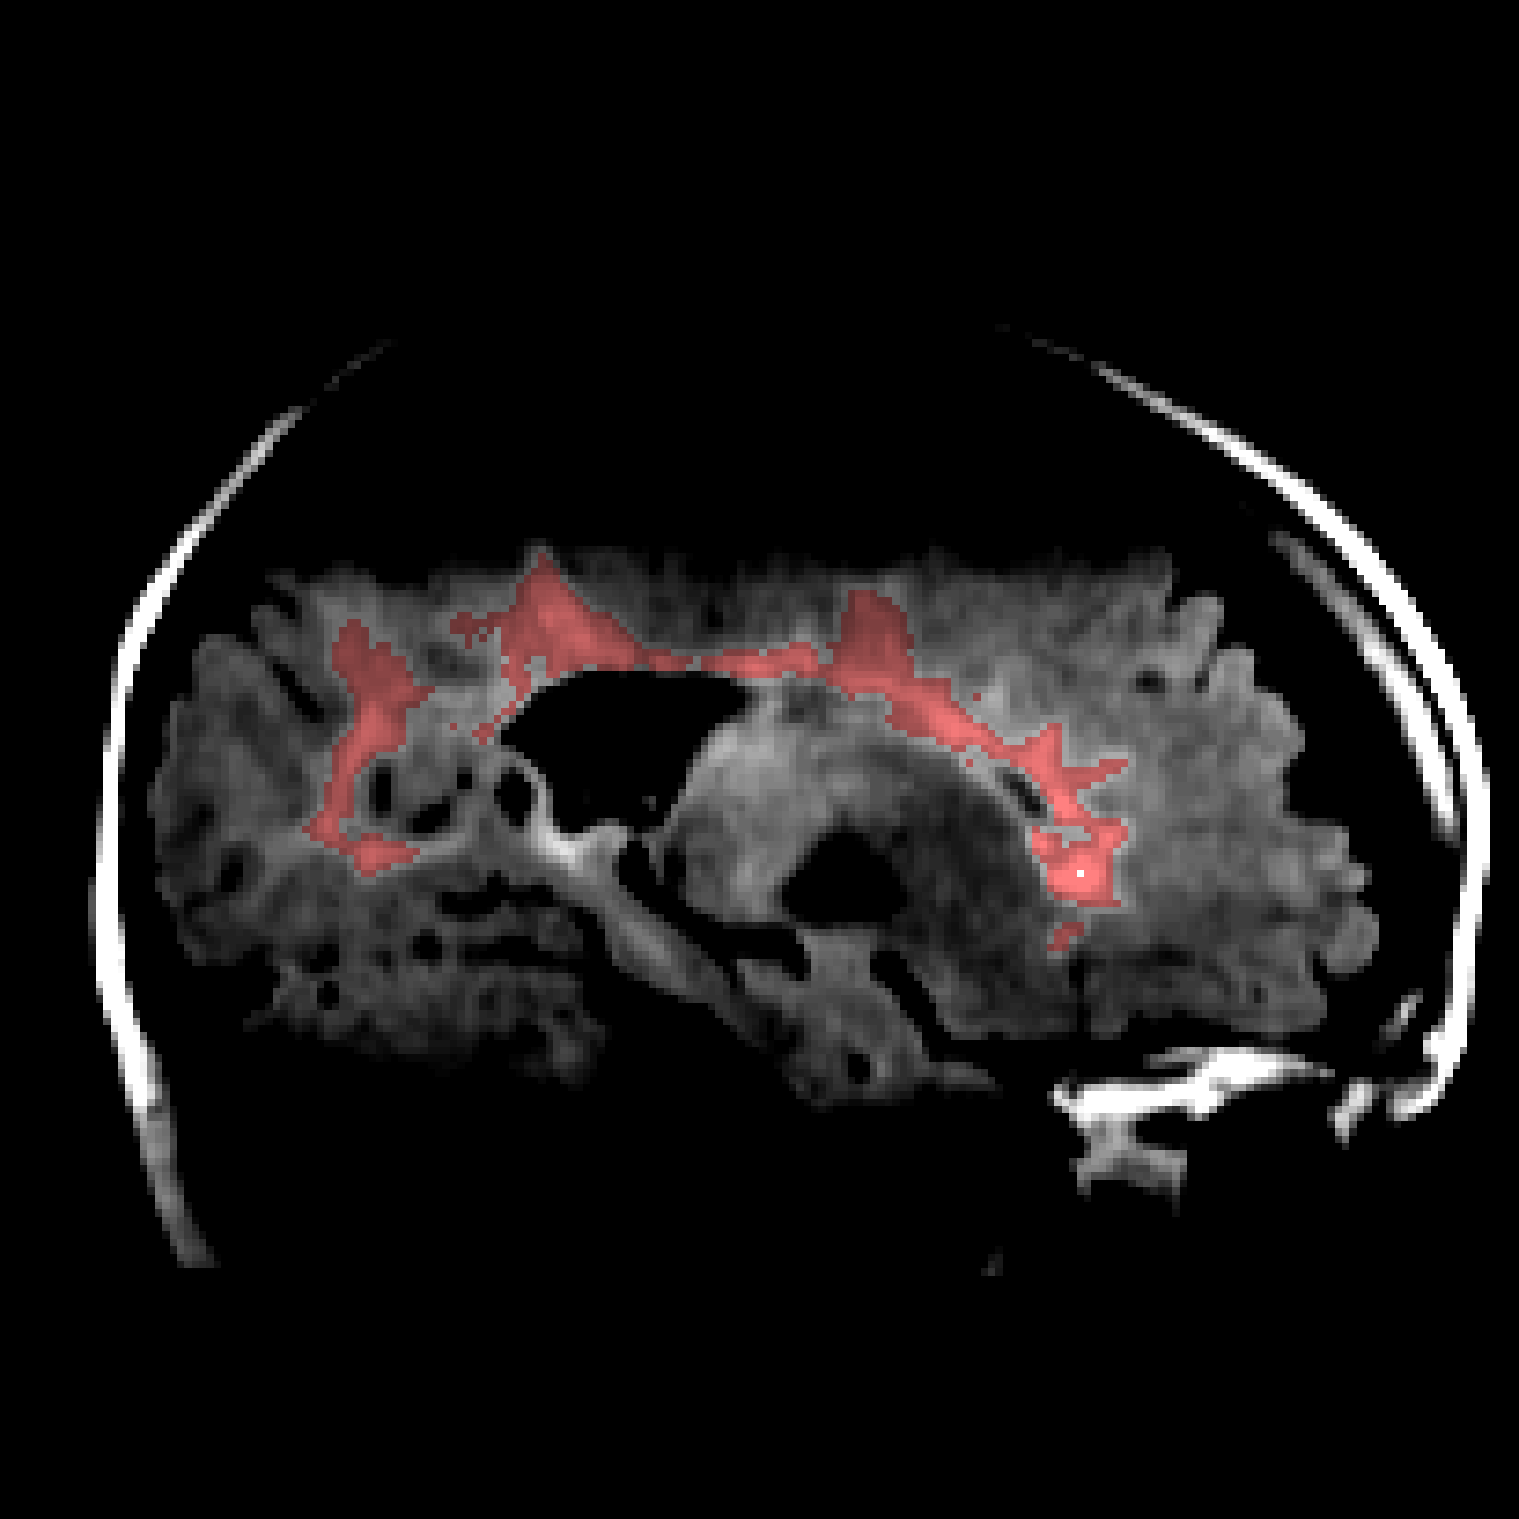
\includegraphics[height=4cm]{m08rev-01-d2-z146-r}\makebox[0pt][r]{\textcolor{white}{ CHB 01 }}
%%    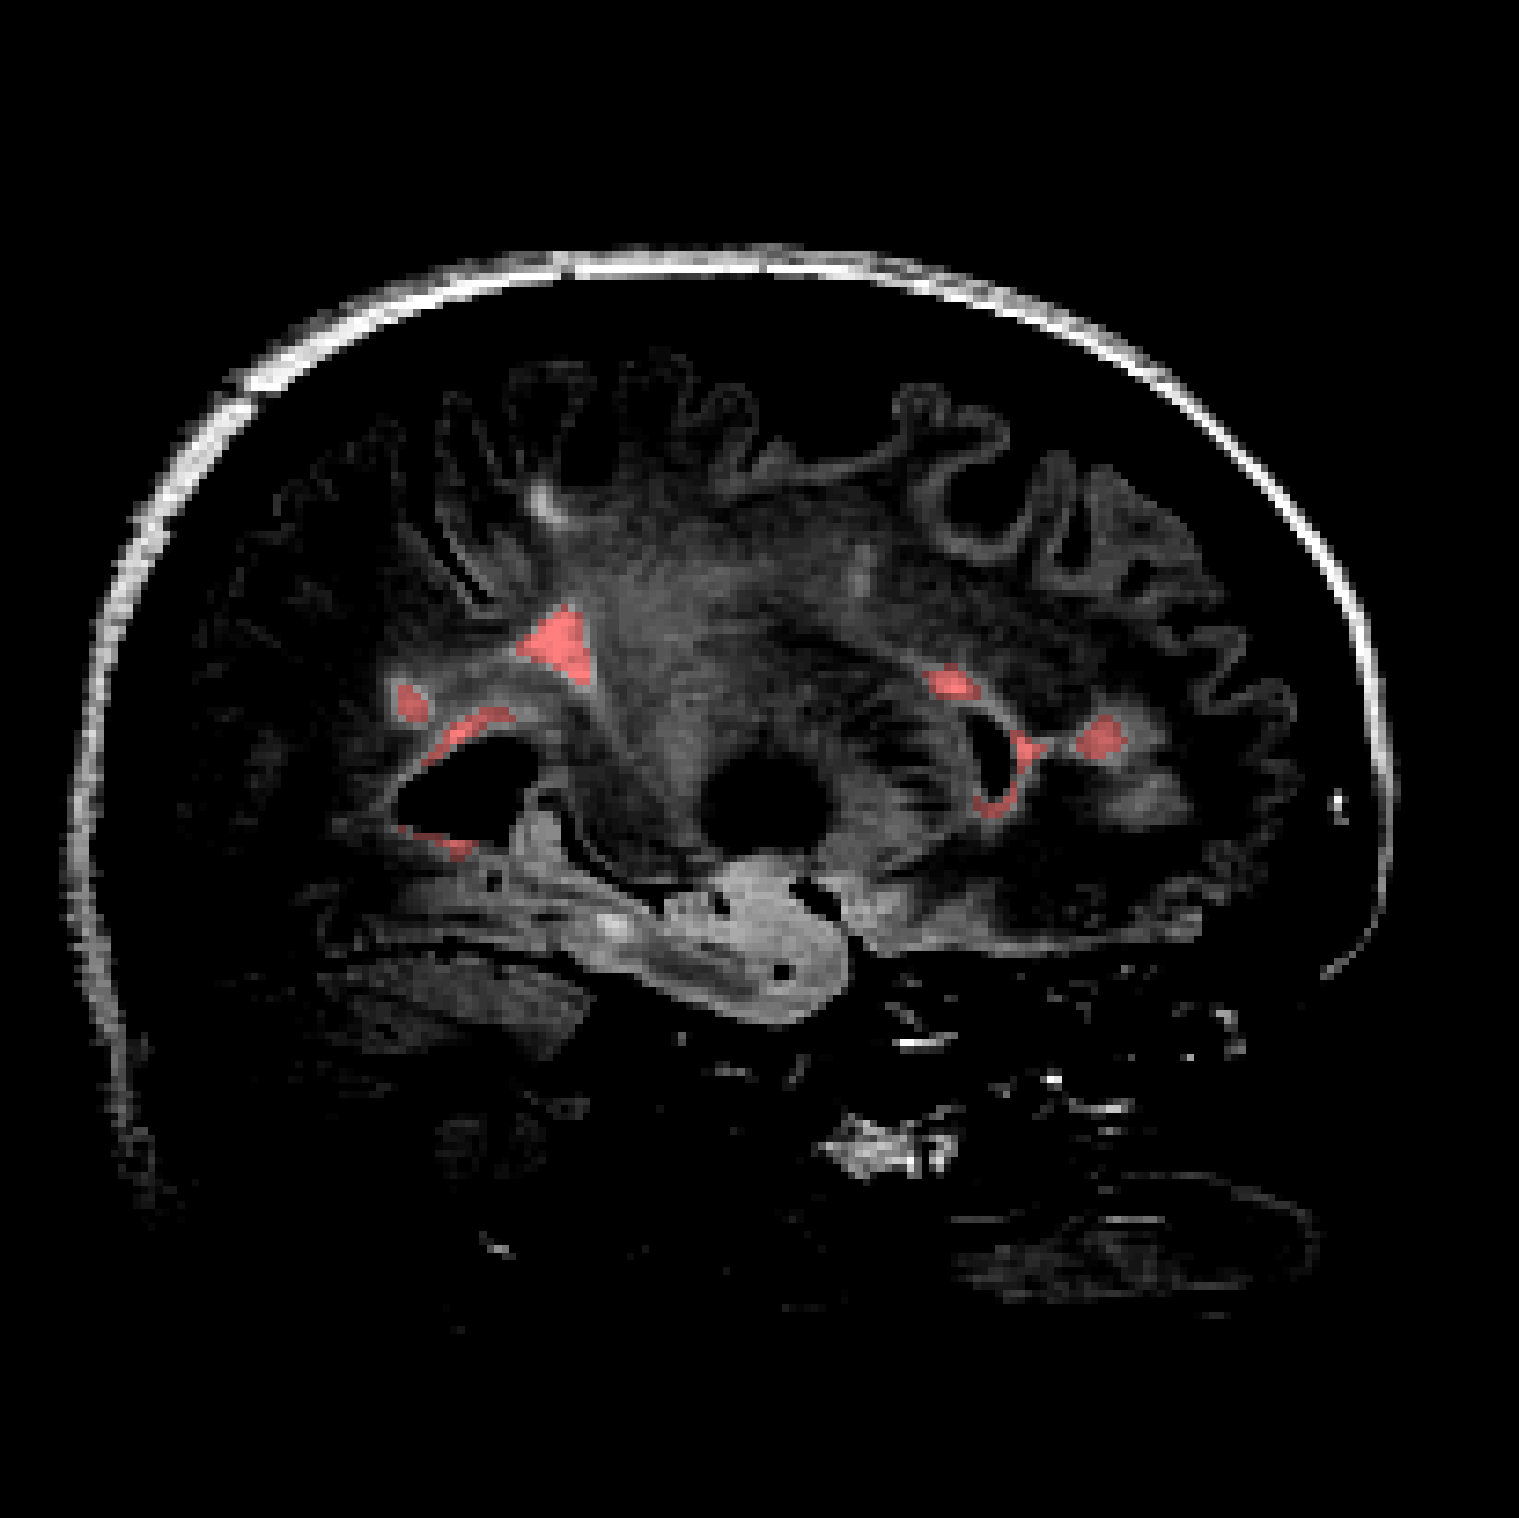
\includegraphics[height=4cm]{m08rev-05-d2-z107-r}\makebox[0pt][r]{\textcolor{white}{ CHB 05 }}
%%    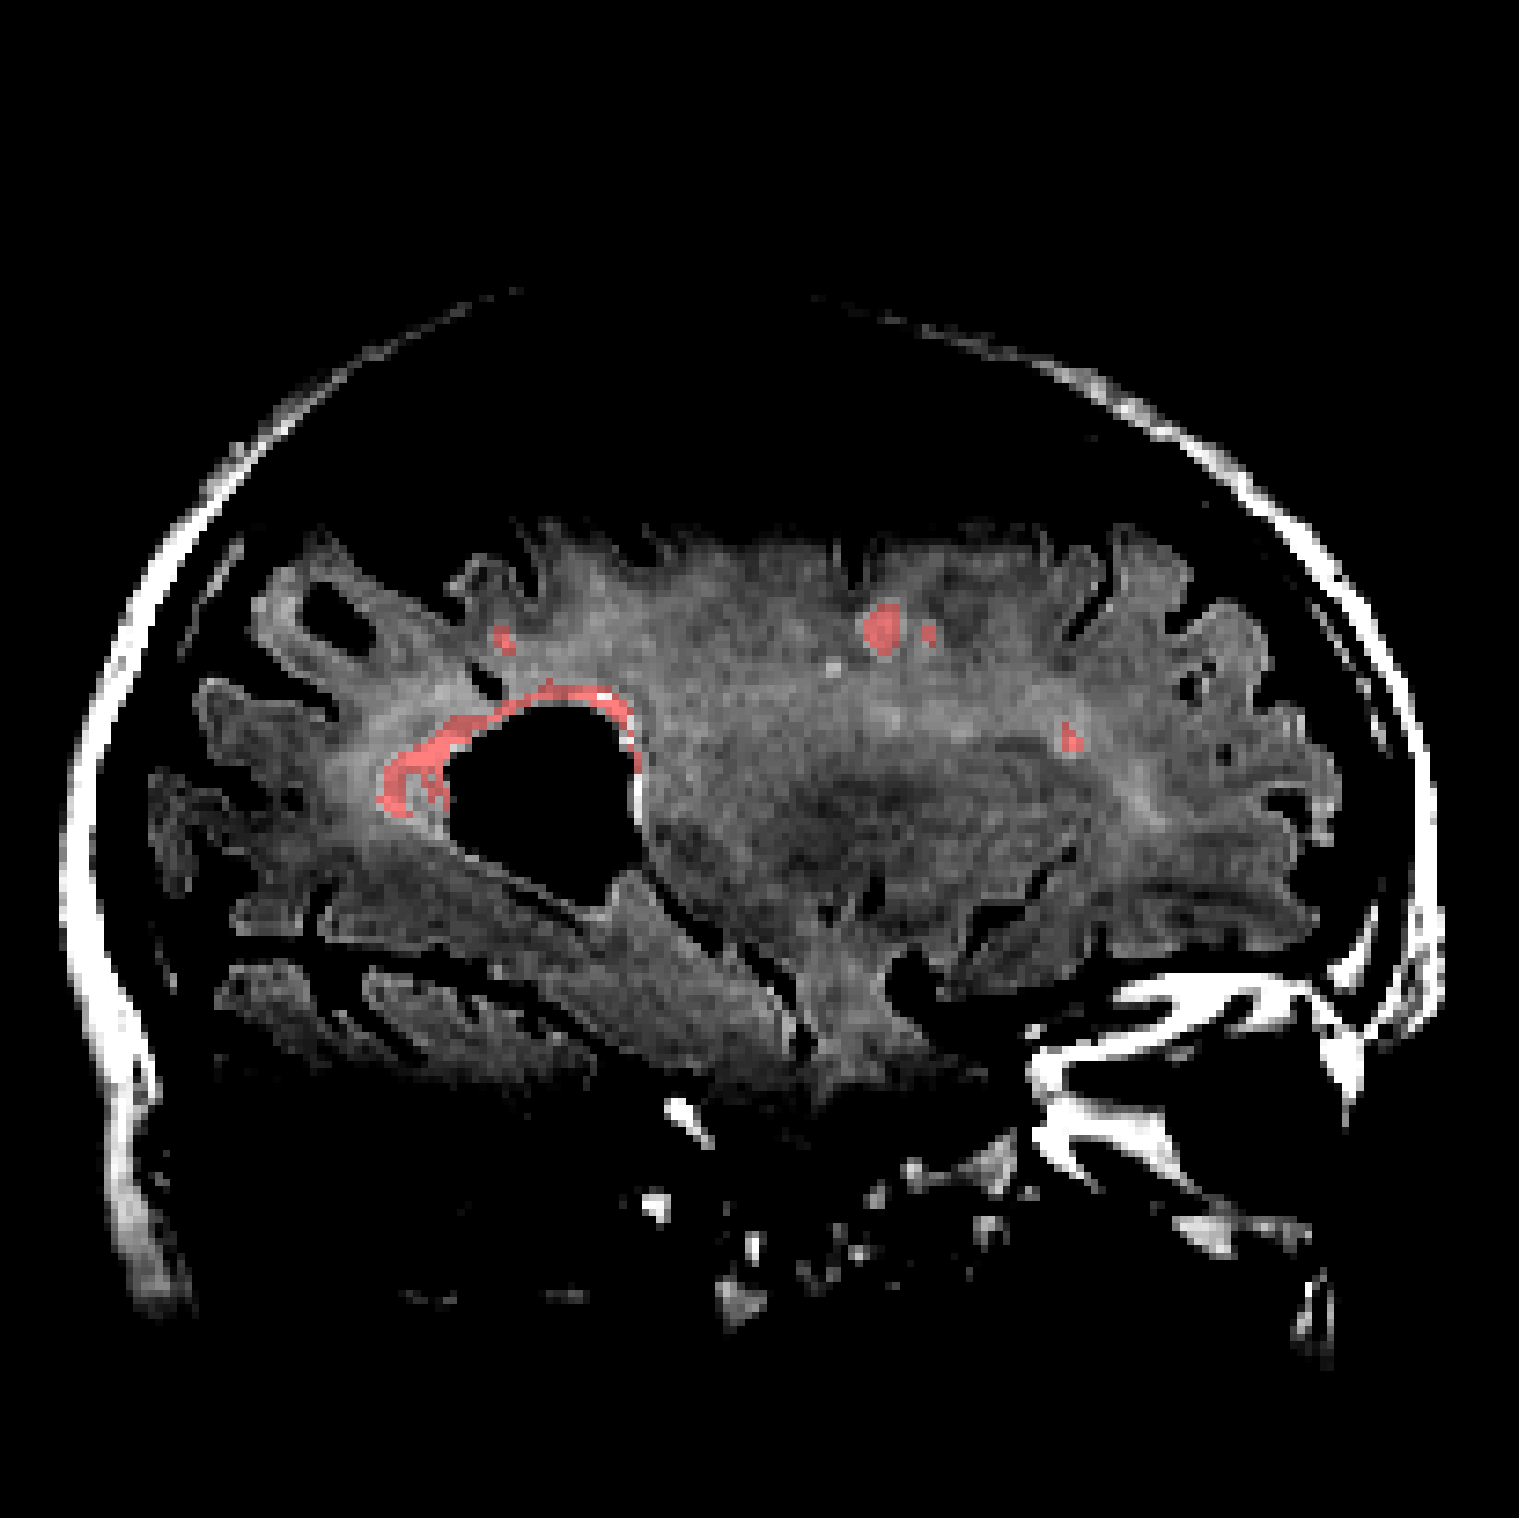
\includegraphics[height=4cm]{m08rev-06-d2-z101-r}\makebox[0pt][r]{\textcolor{white}{ CHB 06 }}
%%  \end{subfigureside}
%  \begin{minipage}{6cm}
%    \begin{subfigure}{\textwidth}
%      \centering\subcaption{Original}\label{fig:m08-rev-o}
%      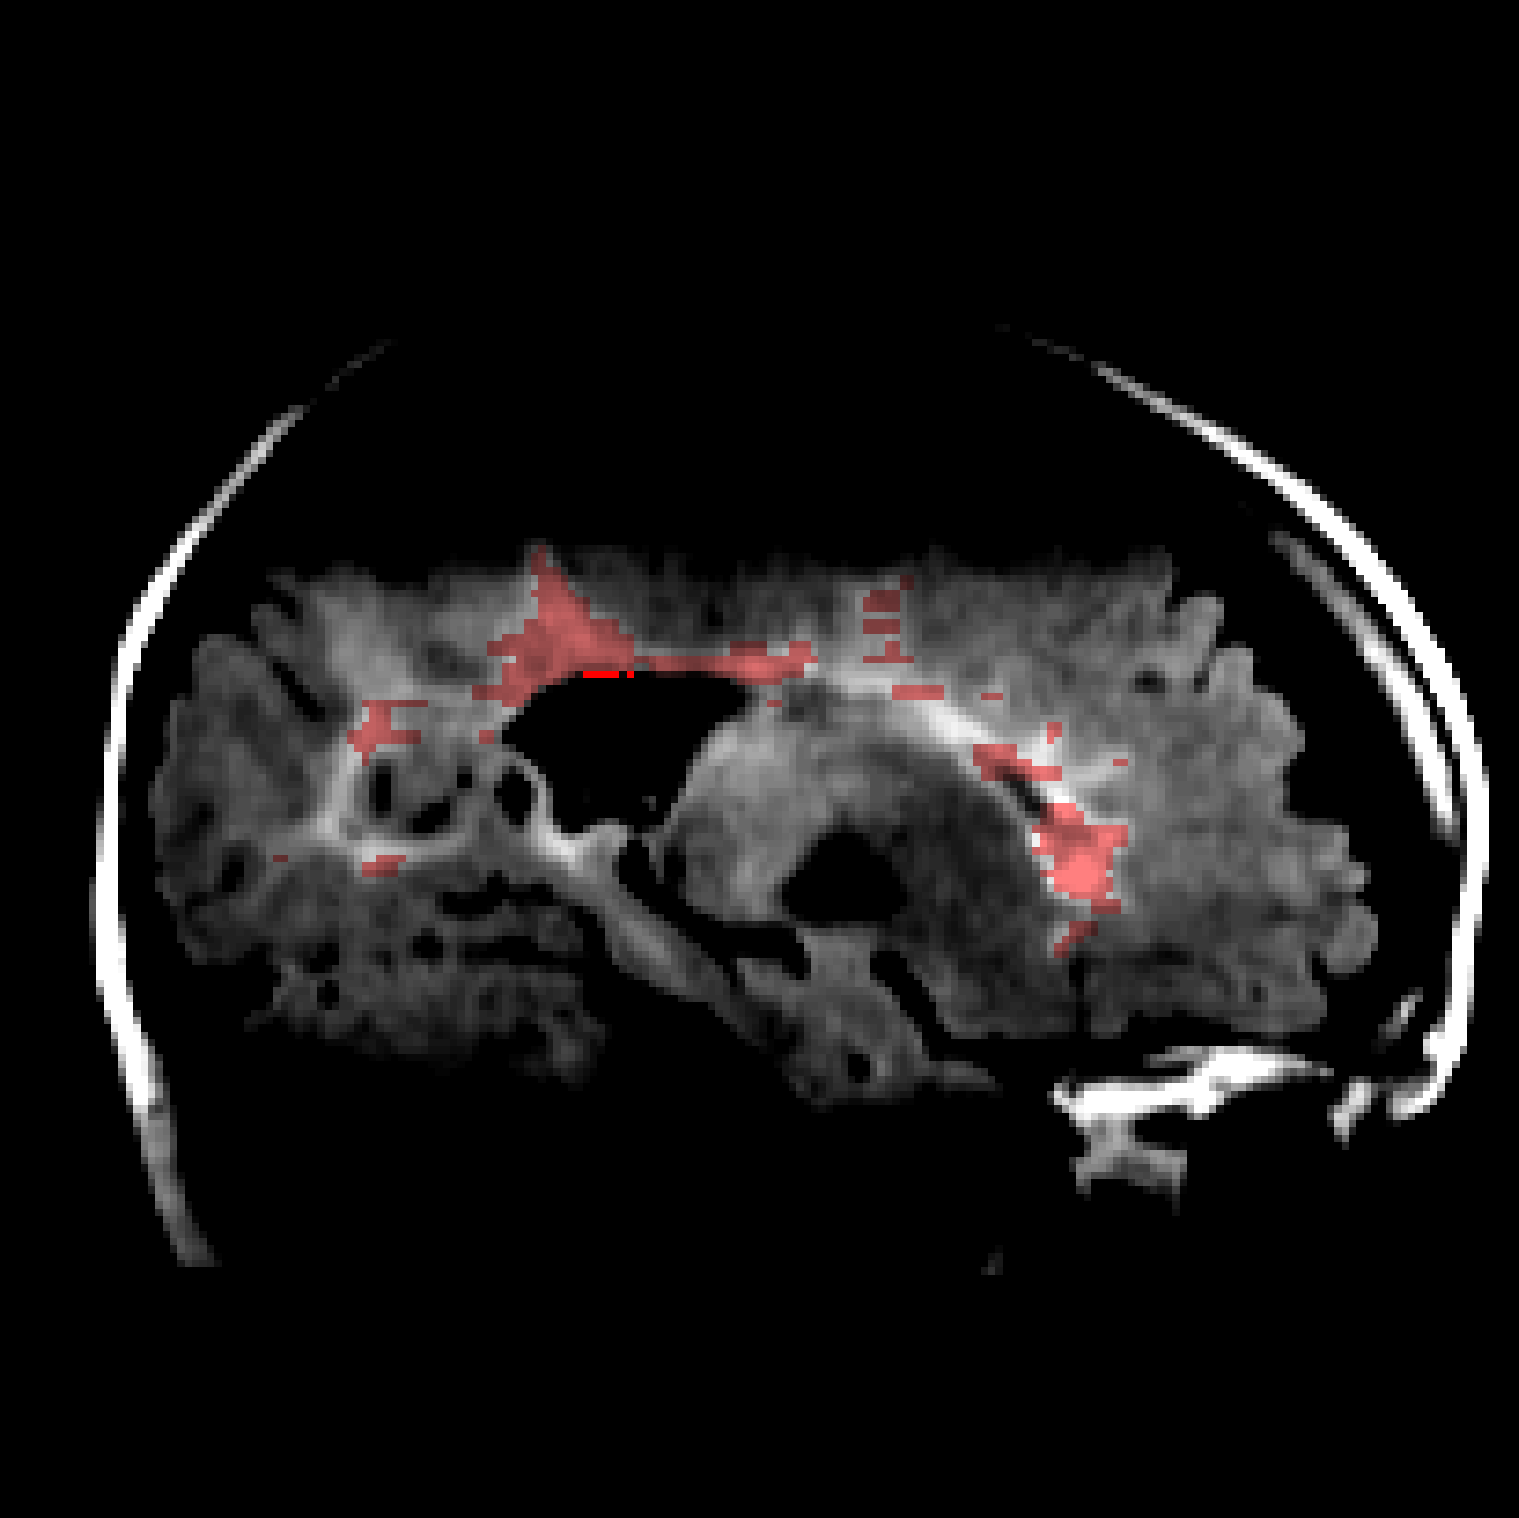
\includegraphics[height=6cm]{m08rev-01-d2-z146-o}\\[0.2em]
%      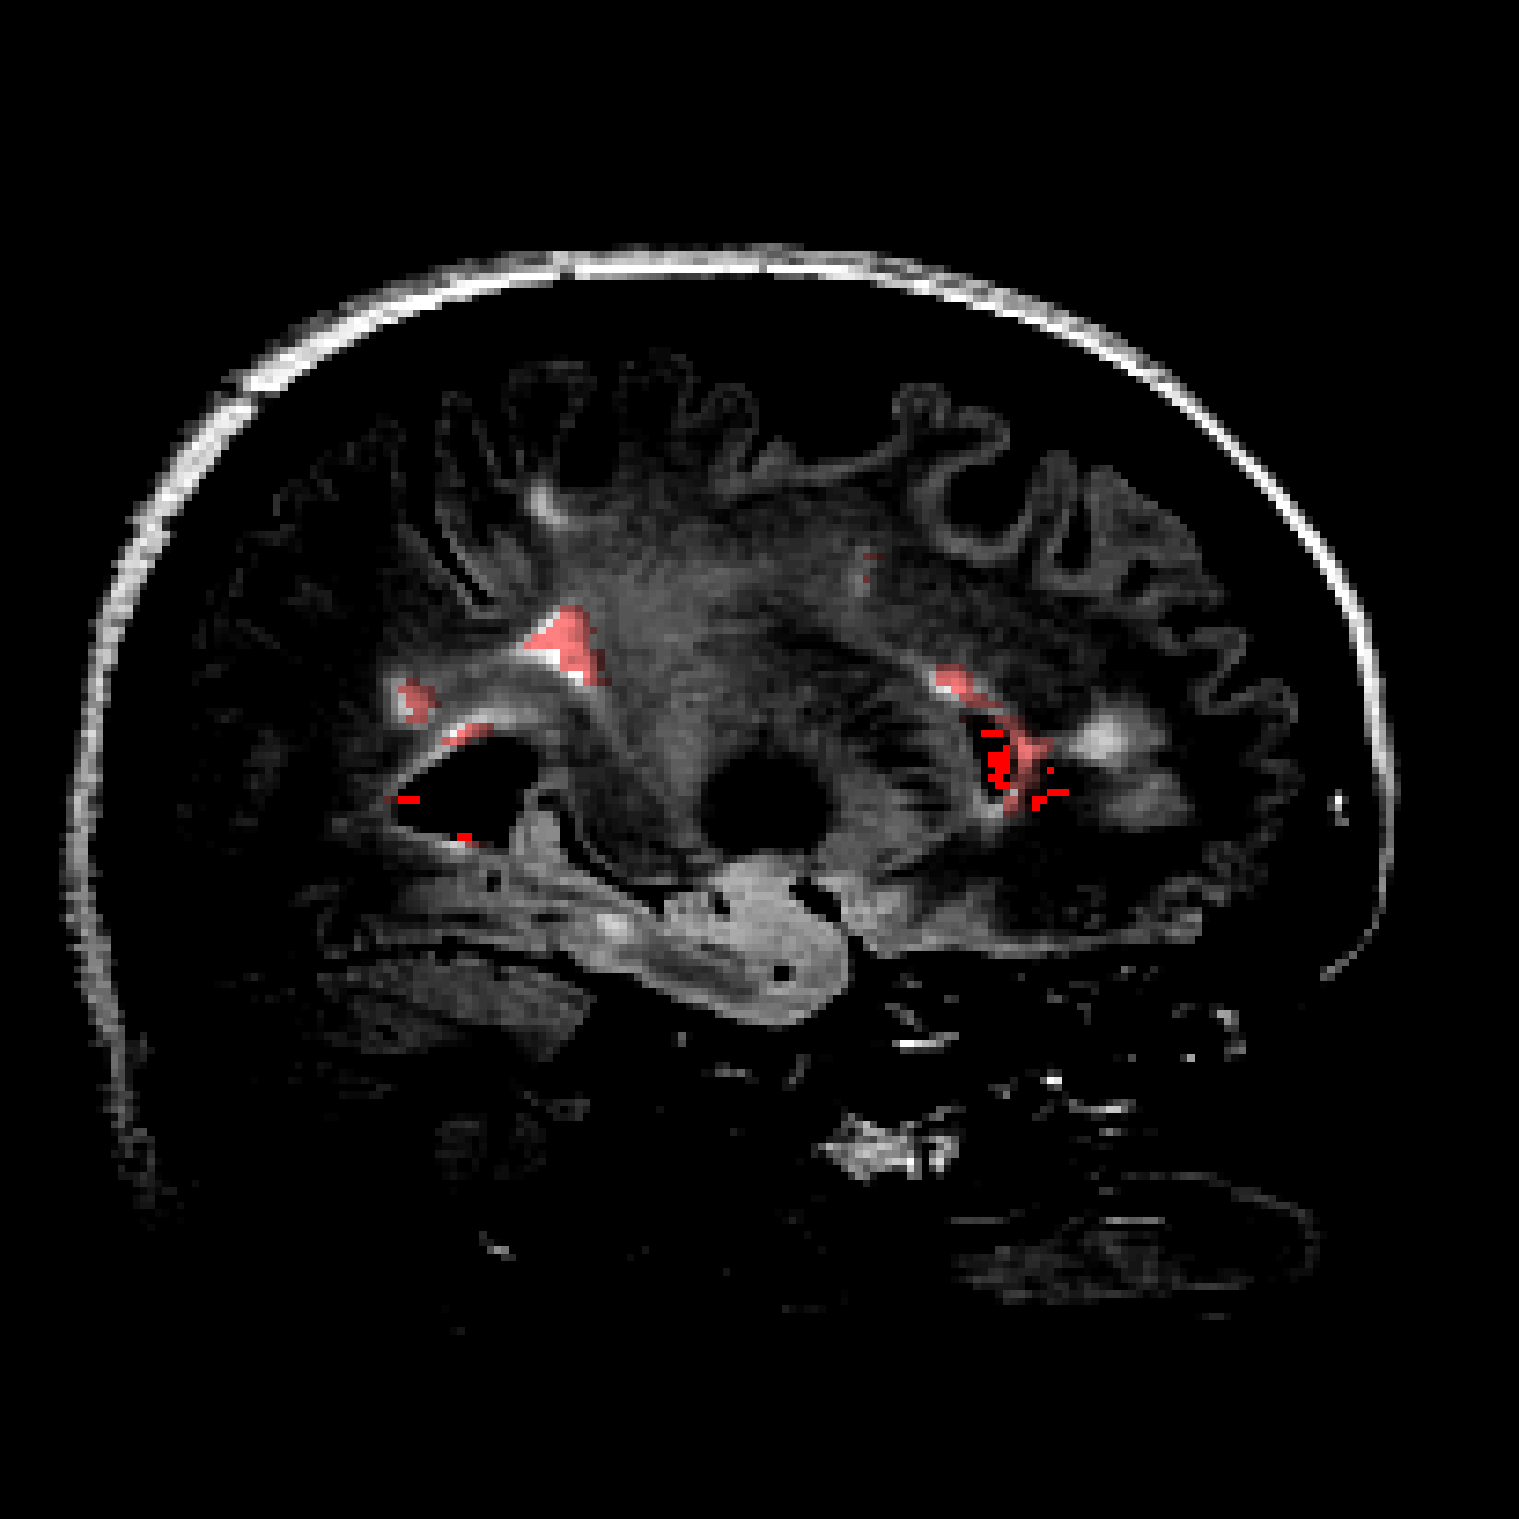
\includegraphics[height=6cm]{m08rev-05-d2-z107-o}\\[0.2em]
%      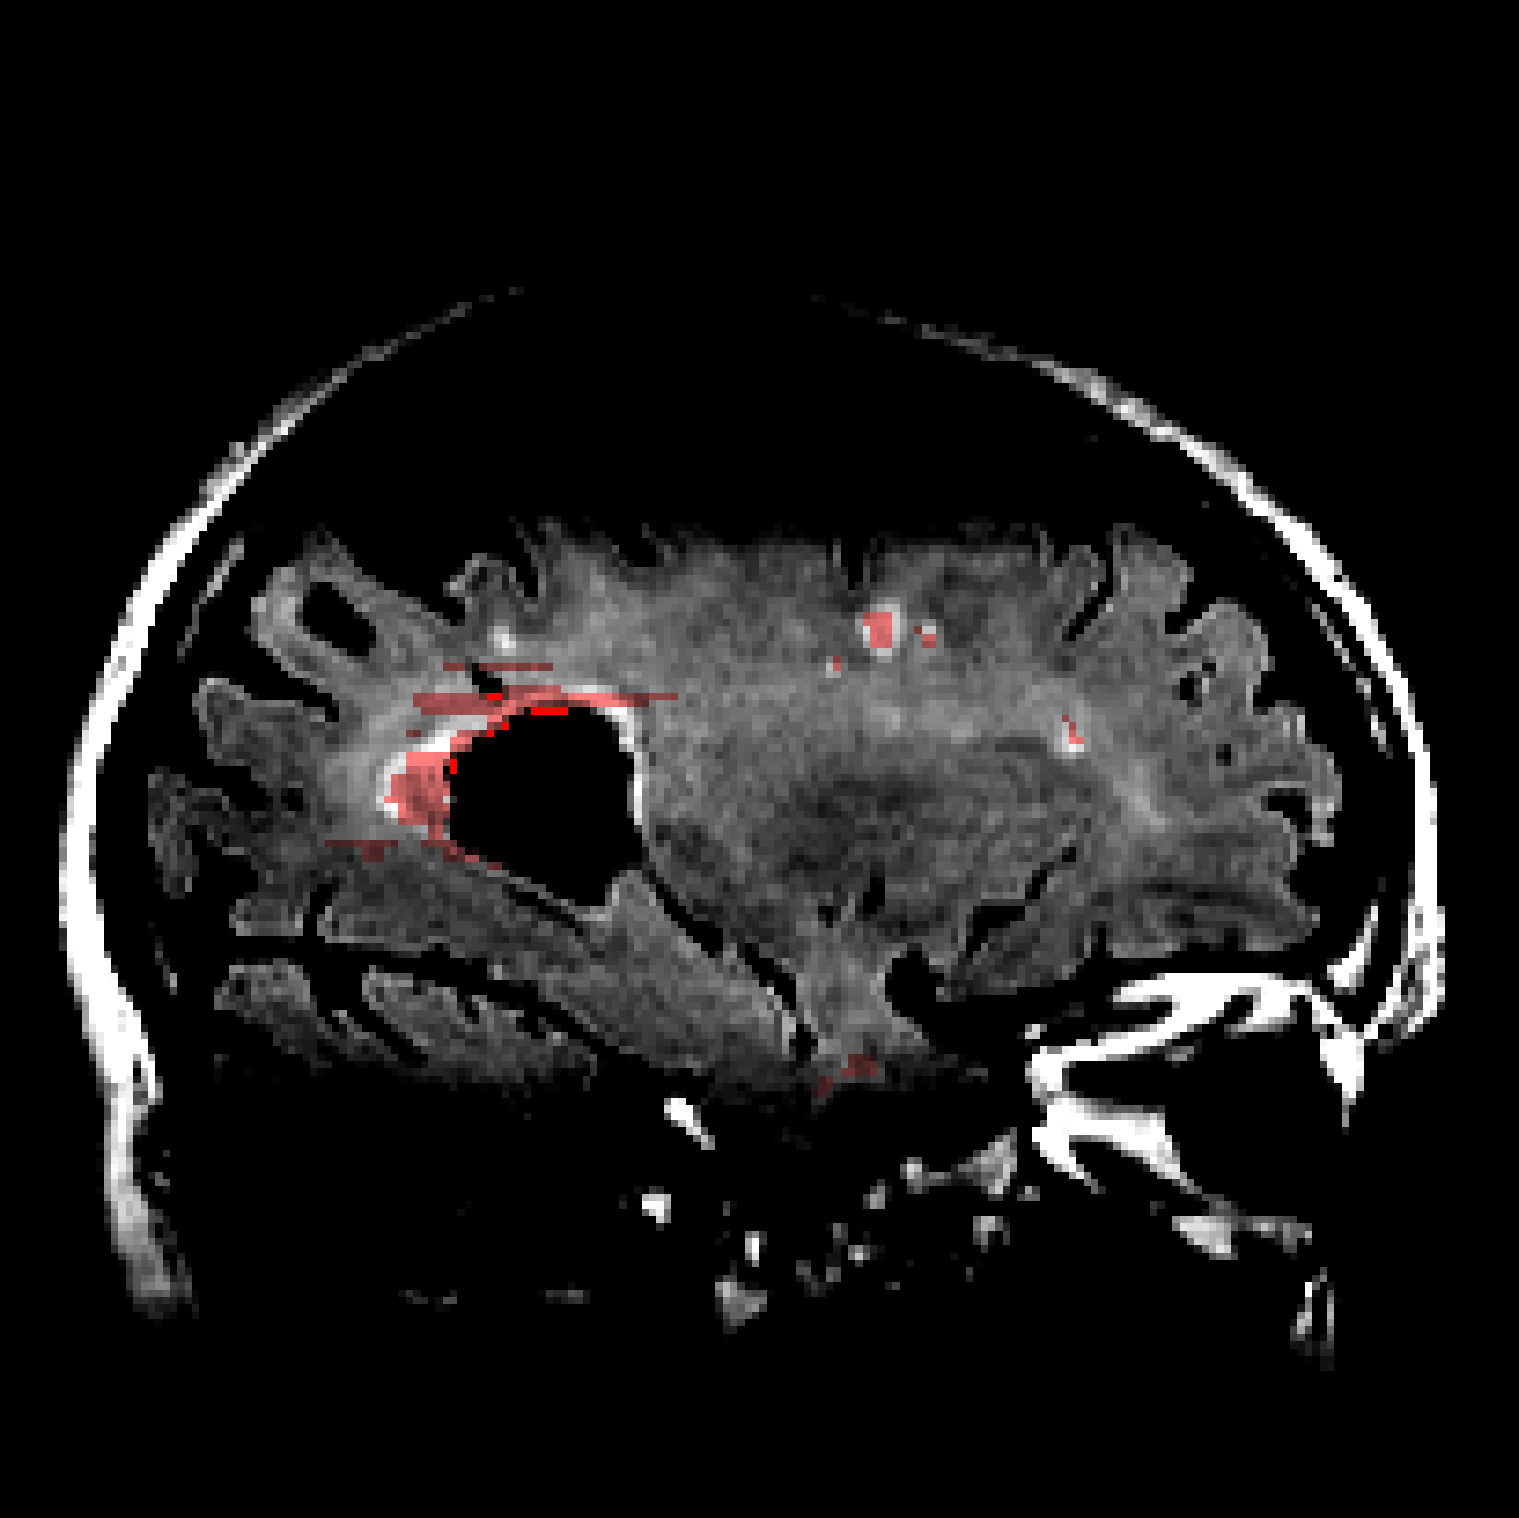
\includegraphics[height=6cm]{m08rev-06-d2-z101-o}
%    \end{subfigure}
%  \end{minipage}
%  \begin{minipage}{6cm}
%    \begin{subfigure}{\textwidth}
%      \centering\subcaption{Revision}\label{fig:m08-rev-r}
%      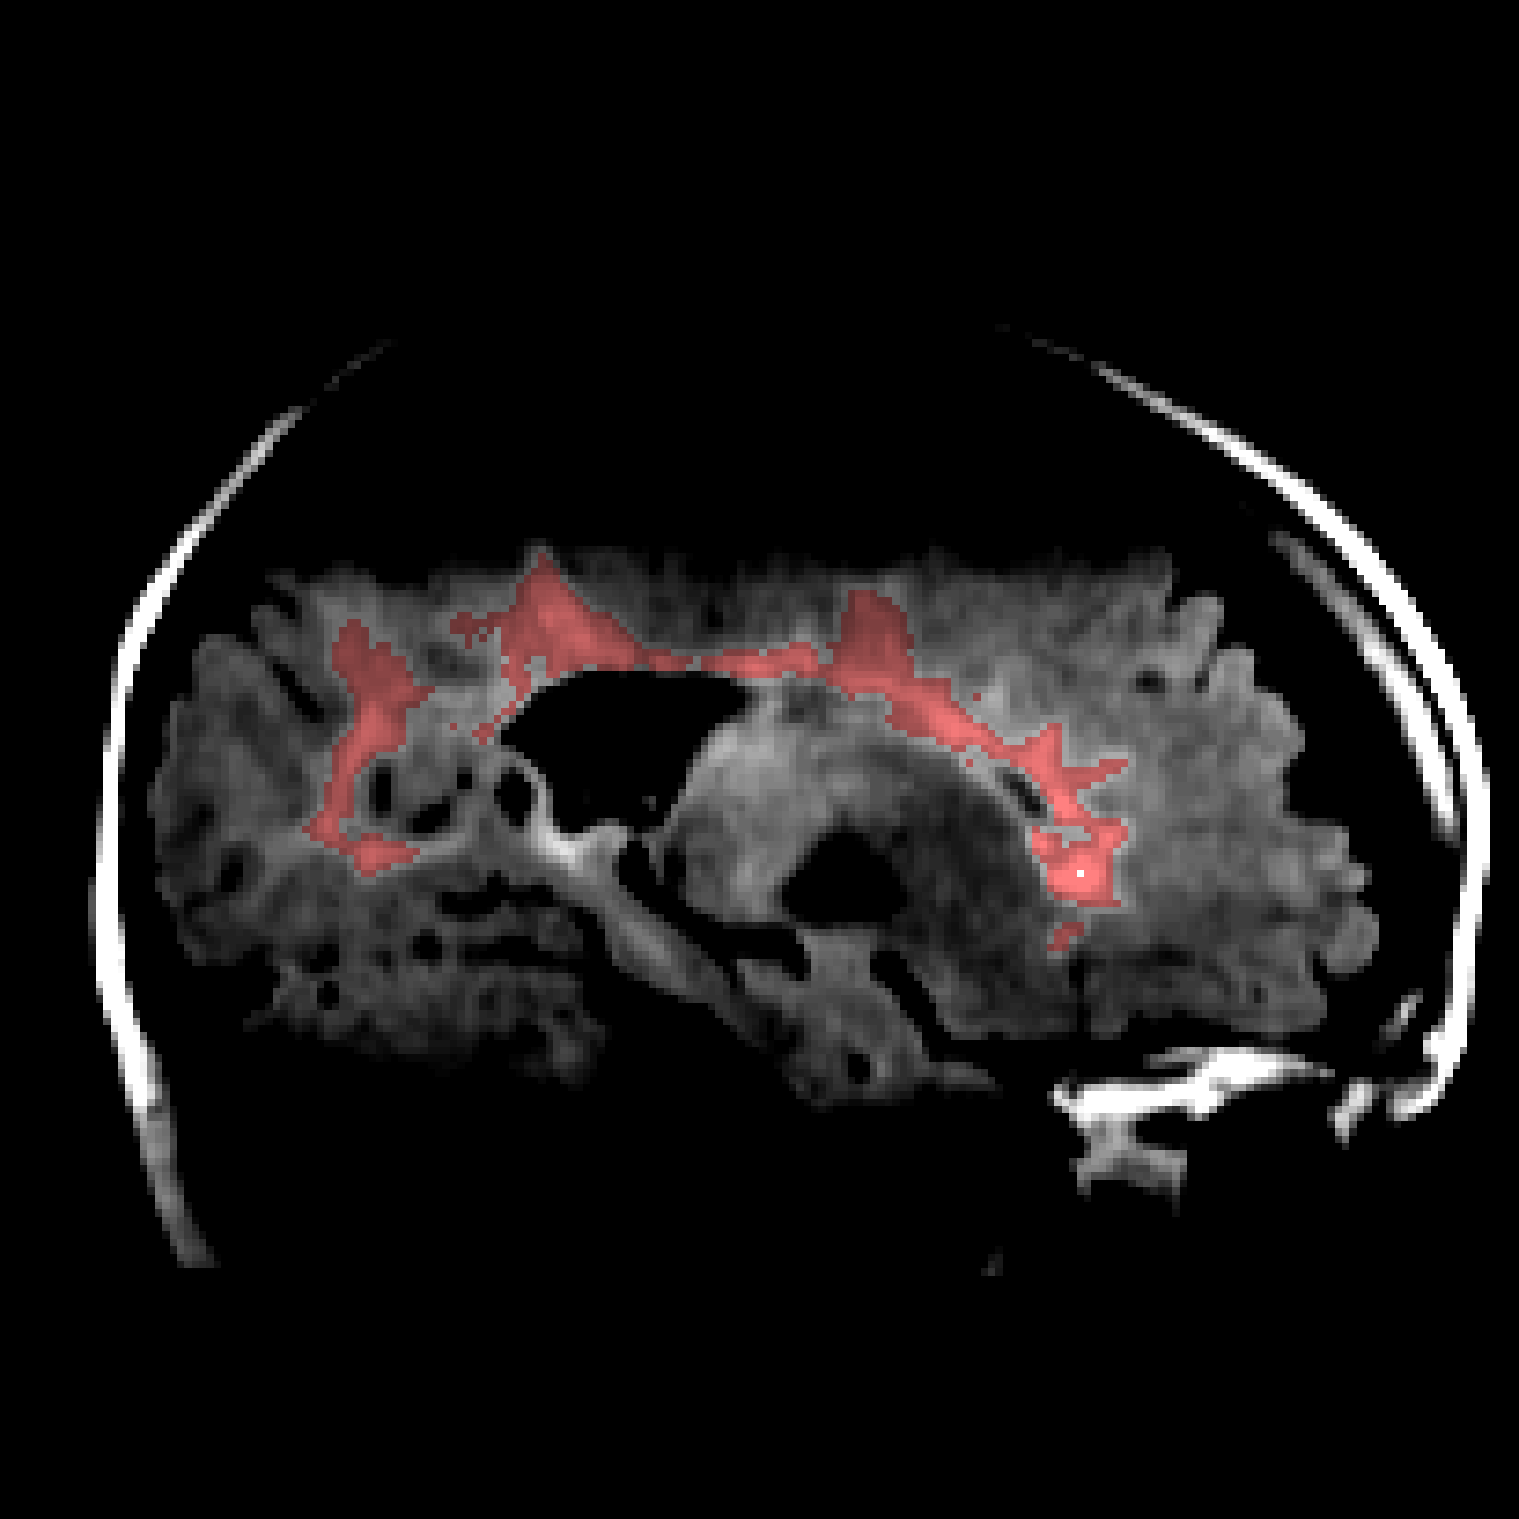
\includegraphics[height=6cm]{m08rev-01-d2-z146-r}\makebox[0pt][r]{\textcolor{white}{ CHB 01 }}\\[0.2em]
%      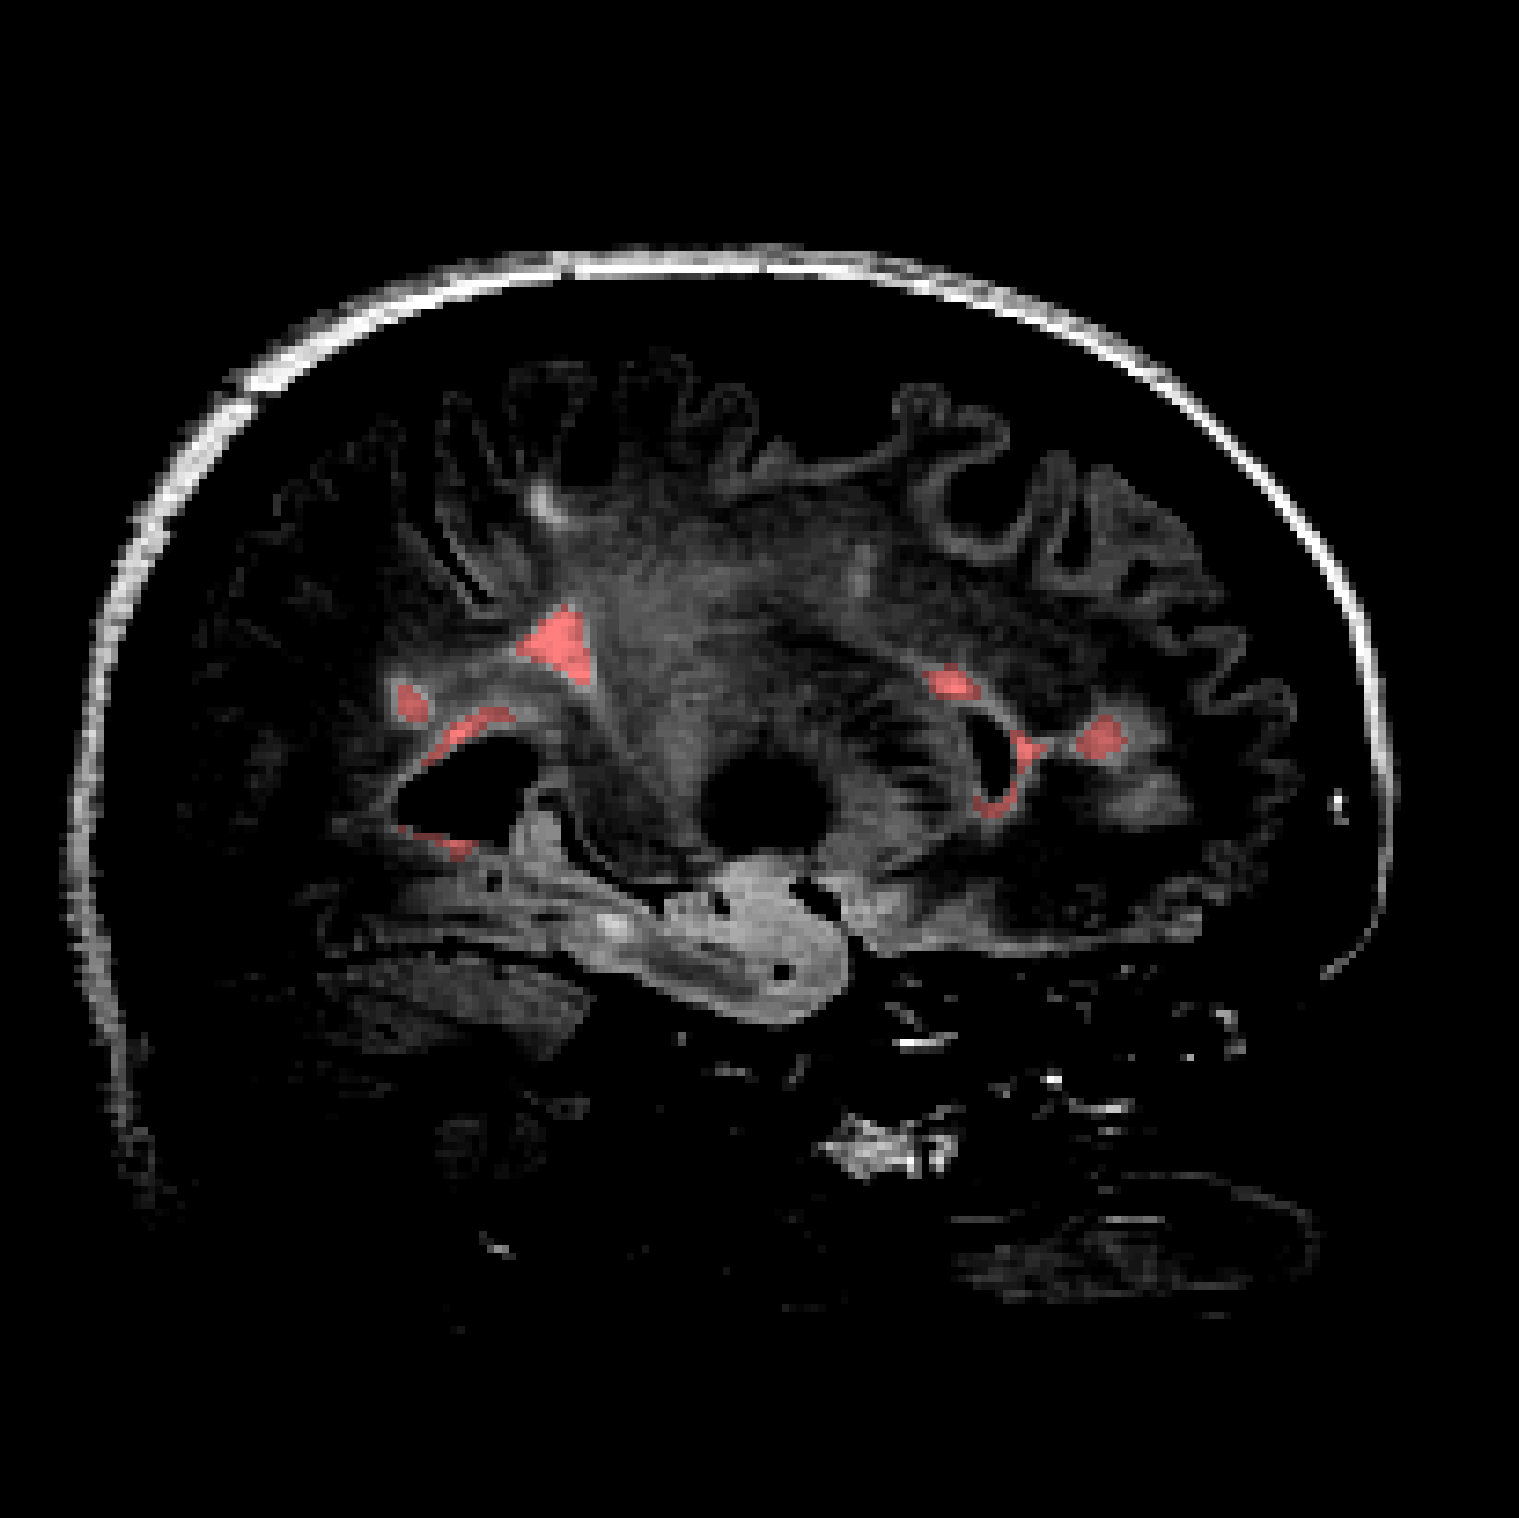
\includegraphics[height=6cm]{m08rev-05-d2-z107-r}\makebox[0pt][r]{\textcolor{white}{ CHB 05 }}\\[0.2em]
%      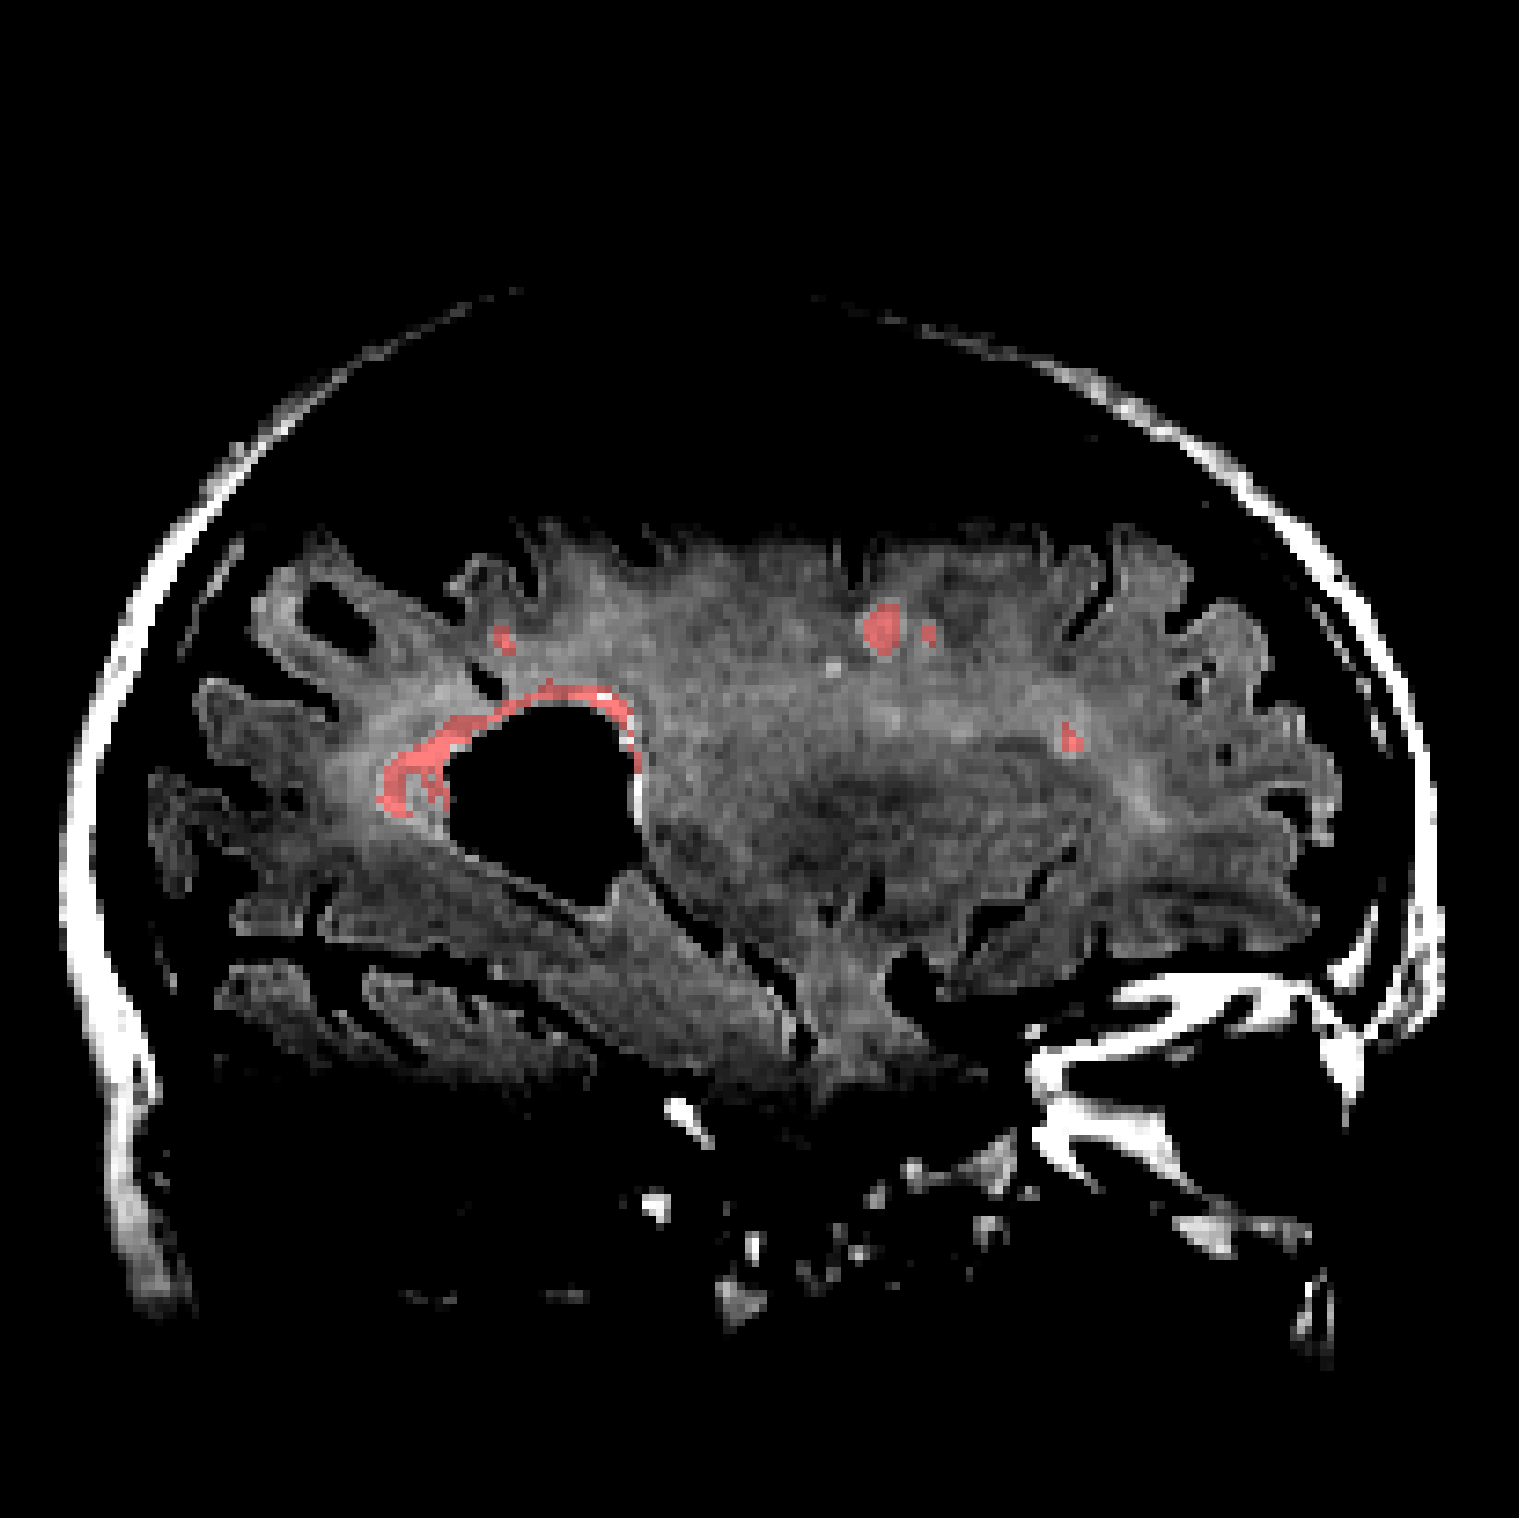
\includegraphics[height=6cm]{m08rev-06-d2-z101-r}\makebox[0pt][r]{\textcolor{white}{ CHB 06 }}
%    \end{subfigure}
%  \end{minipage}
%  \caption{Example revisions to the manual segmentations for the MS 2008 challenge dataset.}
%  \label{fig:m08-rev}
%\end{figure}
% ---
%\clearpage
%\includecode{hypdef.m}
% ---
%\begin{align}
%\bb^T\by &= \b^0 + \b^1 y^1\nonumber\\
%&= s(y-\tau) \qquad\begin{cases} s = \b^1\\ \tau = -\frac{\b^0}{\b^1} \end{cases}.
%\label{eq:reparameterize}
%\end{align}
% ---
\end{document}